\documentclass[onefignum, onetabnum,onealgnum,onethmnum, oneeqnum]{siamonline190516}
\input{nd_preamble.tex}  
\usepackage[symbol]{footmisc}
\renewcommand{\thefootnote}{\arabic{footnote}}
\usepackage{ericmath}


\definecolor{fig1green}{rgb}{0.01, .7, 0.1}
\definecolor{fig1orange}{rgb}{0.7, 0.34, 0.005}
\newcommand{\Combat}{\texttt{ComBat}}
\newcommand{\combat}{\texttt{ComBat}}
\newcommand{\cCombat}{\texttt{Cond.}~\texttt{ComBat}}
\newcommand{\ccombat}{\texttt{Cond.}~\texttt{ComBat}}
\newcommand{\cccombat}{\texttt{Causal}~\texttt{cComBat}}
\newcommand{\edits}[1]{{\color{black} #1 }}


\title{
A Causal Perspective for Batch Effects: when is no answer better than a wrong answer?
}

\author{
    Eric W.~Bridgeford$^{1,\dagger}$, 
    Michael Powell$^1$,
    Gregory Kiar$^2$,
    Stephanie Noble$^3$,
    Jaewon Chung$^1$,
    Sambit Panda$^1$,
    Ross Lawrence$^1$,
    Ting Xu$^2$,
    Michael Milham$^2$,
    Brian Caffo$^1$,
    Joshua T.~Vogelstein$^{1}$
    \thanks{
     $^1$ Johns Hopkins University $^2$ Child Mind Institute, $^3$ Yale University,
    $^\dagger$ Corresponding author:
      Eric W.~Bridgeford (\email{ebridge2@jhu.edu}), 3400 N. Charles Street Clark Hall, Suite 200. Baltimore, MD, USA 21218.}
}


\makeatletter
\def\thanks#1{\protected@xdef\@thanks{\@thanks
        \protect\footnotetext{#1}}}
\makeatother
\makeatletter
\renewcommand\@biblabel[1]{#1.}
\makeatother
\begin{document}

\maketitle

\begin{abstract}
\edits{Batch effects, undesirable sources of variance across multiple experiments, present significant challenges for scientific and clinical discoveries. Specifically, batch effects can introduce spurious findings and obscure genuine signals, contributing to the ongoing reproducibility crisis. Typically, batch effects are treated as associational or conditional effects for both detection and harmonization, despite their potential to causally impact downstream inferences due to variations in experimental design and the underlying study populations. In this study, we propose a framework to formalize batch effects as causal effects. We then develop straightforward procedures to augment existing approaches with causal machinery for batch effect detection and correction. We illustrate via simulation that with sufficiently similar data across batches, our causal approaches mitigate spurious findings and reveal additional signals as compared to conditional approaches. We find that unless often inappropriate assumptions hold, conditional procedures can provide misleading, poorly supported, or incorrect answers about the strength or presence of batch effects. Applying our approaches to a large neuroimaging mega-study, we find that juxtaposition of conditional and causal techniques indicates widely disparate estimates of prevalence rates for batch effects, and so-called ``harmonized data'' yield widely different subsequent inference. Together, we believe that this work provides a framework and potential limitations for the collection, harmonization, and subsequent analysis of multi-site scientific mega-studies.}
\end{abstract}

%
% Stephanie comments
% more information on the existing methods
% ground the definitions in the techniques used
% make clear straight up that the crossover effect is best
% 
\section{Introduction}

The 21\textsuperscript{st} century has seen the advent of high-throughput techniques for acquiring data on an unprecedented scale. Collection of these datasets often occurs through consortia using a range of technologies across different sites, requiring data to be brought together by aggregation services and hosted by data banks for storage and sharing. These ``mega-studies'' comprising numerous individual studies serve the useful purpose of facilitating inference on individuals with unprecedented diversity; researchers can subvert traditional sample size and generalizability issues through the use of data from a more diverse sample of the population than could otherwise be collected.

Unfortunately, aggregating data across diverse datasets introduces a source of undesirable variability known as a batch effect. Several strategies have been proposed to define a batch effect. \citet{Lazar2013Jul} summarize many of these approaches succinctly: ``the batch effect represents the systematic technical differences when samples are processed and measured in different batches and which are unrelated to any biological variation.'' Unfortunately, this unified description  provides limited information about how batch effects manifest, nor how they can be formally characterized and investigated. We have been unable to find a satisfactory technical definition of batch effects in the literature. 

{\color{black}Broadly, many approaches model the batch collection or measurement process as a nuisance variable which is to be removed \cite{Pearl2010Jul,Johnson2007Jan,Leek2010-ua,Leek2015-jc,Wachinger2020Feb,Yu2018Nov,Pomponio2020Mar}, which implies  batch effect is a particular component of an associational or conditional model. These approaches typically make strong, potentially unjustified, and often inappropriate parametric assumptions about the data. % Moreover, they are typically limited to Euclidean variables and binary outcomes. 
% 
Two of the most prominent examples of these techniques which can be generalized to many of these other cases are the \Combat~and Conditional \Combat~batch effect correction procedures \cite{Johnson2007Jan}. These approaches have demonstrated empirical utility in certain genomics and neuroimaging contexts~\cite{Zhang2020Sep,Pomponio2020Mar}; however, it remains unclear when these approaches will be successful and when they will fail. Specifically, they could either remove biofidelic variability or fail to remove nuisance variability. }



% These approaches, as we will illustrate below, are effective when the batches have similar demographic distributions. But, it is unclear what are the 
% 
% a lack of studies determining the appropriateness of these assumptions fails to justify their use in numerous contexts, such as neuroimaging. This is incompatible with modern views in many fields, such as causal inference, in which these assumptions are treated as extremely strong (and \textit{potentially prohibitive}) \cite{Rosenbaum1983Apr,Rosenbaum1985,Stuart2010Feb}.
% 
% We believe removing batch effects benefits from first \textit{understanding} batch effects formally. This inconsistency is compounded by the existence of testing approaches that readily apply to testing for differences between two non-Euclidean samples of data, such as the Distance Correlation (\Dcorr) \cite{Szekely2007Dec}, which have not yet been applied for batch effect detection.  This logical inconsistency has led to emphasis on the removal of associational effects or a removal of all systematic variation that exists between batches in a scientific investigation. This is not ideal due to the fact that batches may differ on other impactful variables (e.g., key demographic covariates) that may skew the observed associational heterogeneity. Other approaches remove conditional effects which, while more sophisticated, are also not necessarily appropriate. These strategies remove a batch effect conditional on key demographic covariates thought to impact the observed measurement. This has the limitation that, if the observed populations from which individuals are taken are not similar on the basis of both known and unknown impactful covariates, strong assumptions are required to claim that the conditional batch effect is a faithful representation of the true batch effect. For instance, the revolutionary 


In this work, we develop a unified and systematic approach to the definition, detection, estimation, and mitigation of  batch effects. Our main conceptual advance is appreciating that one can view batch effects as causal effects rather than associational effects.  Given this understanding, we introduce a formal definition of causal batch effects. This formal definition reveals the limitations of (typically inappropriate) assumptions implicit in existing approaches~\cite{Rosenbaum1983Apr,Rosenbaum1985,Stuart2010Feb}. Methodologically, we introduce a simple strategy appended to existing techniques for associational or conditional batch effect detection and removal to reflect this new perspective. 

We demonstrated the utility of this perspective by developing \textit{Causal} \Dcorr~\cite{Szekely2007Dec}---building on modern, non-parametric statistical methods---to estimate and detect the presence of batch effects. Second, we utilized this strategy to develop \textit{Causal} \Combat---an augmentation of the \Combat~procedure---which uses causal methods to remove batch effects while limiting the removal of variation due to known demographic variables. Our main empirical contribution is to apply these methods to simulations and a large neuroimaging mega-study assembled by the Consortium for Reliability and Reproducibility (CoRR) \cite{corr}, consisting of more than $1700$ connectome measurements across $27$ disparate studies. Our investigations reveal that previous strategies fail to differentiate between veridical signal and sources of variability due to other experimental design factors. Further, our simulations demonstrate that existing strategies can, under many realistic use-cases, remove more apparent veridical biological signal (or, struggle to remove the batch effect entirely) than \textit{Causal} \Combat.

{\edits{Informally, these results can be summarized succinctly: when upstream covariate distributions of measured individuals vary widely, and those covariates are known to impact both the measurements and the selection of individuals to particular batches (the covariates are confounding), parametric techniques can yield imprecise estimates of batch effects. Through simulation, we illustrate that causal adjustments to these procedures can be used to overcome these limitations. Our real data analysis reveals two salient points:
\begin{enumerate}[leftmargin=*]
    \item strategies to detect batch effects from mega-studies may struggle to parse differences between batch effects and real demographic variability when datasets are insufficiently similar, and
    \item caution must be taken while interpreting the data for subsequent tasks, as upstream procedures (used to mitigate batch effects) directly influence subsequent conclusions. This the challenge of performing principled statistical inference while pooling data from large consortium studies.
\end{enumerate}
Together, we hope this work contributes to the ongoing effort to improve the validity and reliability of inferences in past and future mega-studies.}}

% Specifically, we make the following contributions:
% 
% \begin{enumerate}[leftmargin=*]
% \item We explicitly introduce a formal definition of batch effects leveraging ideas from causal inference. This formal definition reveals the limitations of (typically inappropriate) assumptions implicit in existing approaches~\cite{Rosenbaum1983Apr,Rosenbaum1985,Stuart2010Feb}.
% \item Given this definition, we develop \textit{Causal} \Dcorr~\cite{Szekely2007Dec}, building on modern non-parametric statistical methods, to estimate and detect the presence of batch effects. 
% \item We develop \textit{Causal} \Combat, an augmentation of the \Combat~procedure, which uses causal methods to remove batch effects while limiting the removal of variation due to known demographic variables.
% \item We apply  these strategies to a large neuroimaging mega-study assembled by the Consortium for Reliability and Reproducibility (CoRR) \cite{corr}, consisting of more than $1700$ connectome measurements across $24$ disparate studies. Our investigations reveal that previous strategies fail to differentiate between veridical biological signal and sources of variability due to other experimental design factors. Further, previous strategies for removing batch effects remove more apparently veridical biological signal than  \textit{Causal} \Combat.
% \end{enumerate}
% has been applied to present biological investigations in which establishment of causal batch effect estimands cannot or has not been achieved. 
% \textit{Internal validity} refers to the degree to which evidence supports a claim within the study population being investigated, and \textit{external validity} refers to the degree to which evidence supports broader conclusions which can be applied outside the study population being investigated. 
% Together, we believe t
% This focus on batch effects as a problem in causal inference will transform the manner in which both aggregation and downstream inference on mega-studies is performed.


\input{Content/novel_methods}

\section{Results}
\label{sec:results}
\subsection{Traditional approaches fail to adequately remove batch effects when covariate overlap is poor}
\label{sec:results:sims}
We constructed simulations to help us understand the differences between associational or conditional reasoning and causal reasoning. To this end, we evaluate the performance of our proposed technique, \cccombat, in comparison with two conditional approaches one may use for batch effect correction, including \ccombat~\cite{Johnson2007Jan} and \combatgam~\cite{Pomponio2020Mar}, which leveraged generalized additive models (GAMs) to capture non-linear trends related to age.

Figure \ref{fig:sim_nlin_adjust}(A).I. shows a simulation where the outcome of interest (e.g., a feature of a connectome, $y$-axis) is associated with a covariate of interest ($x$-axis) through a non-linear relationship (the sigmoid). If samples are from the blue batch, they are offset $1$-unit higher than samples from the orange batch. $N=500$ samples are drawn with equal probability from each batch. In the high overlap regime, the orange and blue batches have the same covariate distribution. Figure \ref{fig:sim_nlin_adjust}(B).I. shows the expected signal (solid line) for each batch, along with the difference between the expected signal for each batch (gray box). These curves are shown along with the group-specific linear model fit (dashed lines) estimated from the sample points, which is the model that is later used by \ccombat~for batch effect adjustment. Figure \ref{fig:sim_nlin_adjust}(C).I. and Figure \ref{fig:sim_nlin_adjust}(D).I. show the impact that \ccombat~and \cccombat~have on the expected signal at a given covariate level. Intuitively, one would anticipate that a batch effect correction strategy should place the expected signals virtually overlapping after correction, since the batch effect is characterized by the expected signals in each group differing by an offset factor. For both strategies, the expected signal after correction is virtually the same for each of the two batches, indicating that the batch effect has been successfully removed. \edits{We compute the mean average absolute difference (AAD) across included covariate values of the two lines over $R=1$,$000$ trials, where a mean AAD of $1$ corresponds to the residual disparity on average equaling the original batch effect, and a mean AAD of $0$ corresponds to no residual disparity. The mean AAD is discussed in Appendix \ref{app:maad}. We find that \ccombat~has a mean AAD of $.058$, and \cccombat~a  mean AAD of $.047$, with \cccombat~having a lower mean AAD about $62\%$ of the time.}

Figure \ref{fig:sim_nlin_adjust}(A).II. shows similar plots; however, the covariate distributions have been shifted such that they no longer overlap perfectly. The orange batch has a left-shifted covariate distribution, and the blue batch has a right-shifted covariate distribution (the covariate is \textit{confounding} the relationship between the outcome and the batch). Figure \ref{fig:sim_nlin_adjust}(B).II. shows that while the expected signal in each batch at a given covariate level is the same as in Figure \ref{fig:sim_nlin_adjust}(B).II., the linear model fits for each group estimated from the sample now differ (the lines are rotated slightly in a clockwise direction, and are now offset further apart). Figure \ref{fig:sim_nlin_adjust}(C).II. shows that after correction, the expected signal at each covariate level do not overlap; in fact, they differ more after correction than before. This is because the model being employed by \ccombat~is biased under the given true data distribution. Figure \ref{fig:sim_nlin_adjust}(D).II. shows that, unlike \ccombat, \cccombat~restricts inference to the region of shared covariate overlap between the two batches, and does not perform inference that is unsupported by the data. This is indicated by the fact that the expected signal after correction has been restricted to no longer include the left-most and right-most portions of the covariates. Within this region, the expected signal for each batch after correction are much closer, indicating that the batch effect has been nearly entirely removed after \cccombat. \edits{Over all trials, we find that \ccombat~has a mean AAD of $1.04$, and \cccombat~a mean AAD of $0.22$, with \cccombat~always having a lower mean AAD.}

Figure \ref{fig:sim_nlin_adjust}(A).III. has furthered this trend such that there are almost no samples in a region of shared covariate overlap between the two batches. In Figure \ref{fig:sim_nlin_adjust}(B).III. the expected signal in each batch at a given covariate level is the same as in Figure \ref{fig:sim_nlin_adjust}(B).I., but the per-group linear model fits are now even further offset. \edits{This has the effect that in Figure \ref{fig:sim_nlin_adjust}(C).III., the expected signal after correction has a mean AAD of $3.03$, exceeding the original batch effect by over $200\%$.} On the other hand, \ref{fig:sim_nlin_adjust}(D).III. shows that \cccombat~would indicate to not perform inference at all on the batches due to the fact that there are no portions of the covariate range in which the two batches have samples which could be compared. \edits{\cccombat~only executes on $26$ of the trials, and has a mean AAD of $0.369$, always lower than that of \ccombat~for trials in which it could be executed.}

\begin{figure}[h]
    \centering
    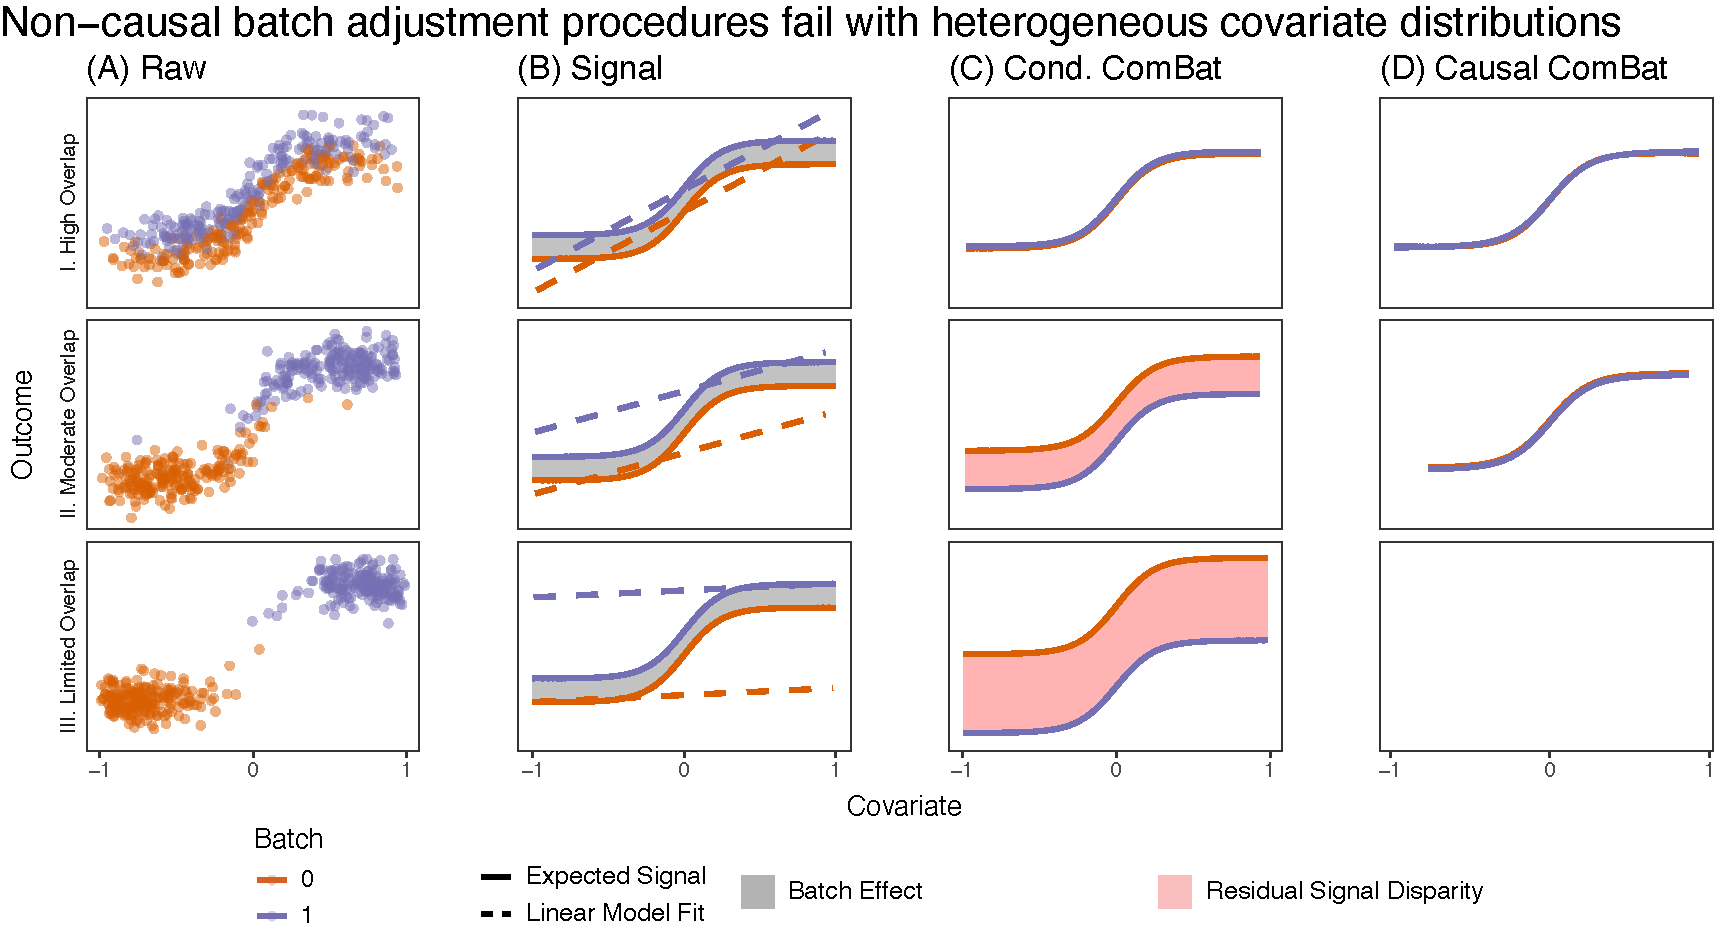
\includegraphics[width=\linewidth]{Figures/Content/sim_nlin_adjust.pdf}
    \caption{\textbf{Non-causal procedures are subject to strong biases without covariate matching}. $N=400$ points are simulated from either batch $0$ or batch $1$ in (A). In (B), the expected signal at a given covariate level is indicated by the solid lines. The batch effect is the difference between the two solid lines (gray box). The estimated linear model fit employed by \ccombat~is indicated with the dashed line. After adjustment (C. and D.), the original expected signal relationship is passed through the trained model, and any residual difference between the true signals of the two batches is termed a residual signal disparity (red box). When coverlap overlap is high in I, both \ccombat~and \cccombat~remove the batch effect successfully, and the expected signal after correction accurately overlaps. With moderate covariate overlap in II, the limitations of the \ccombat~model introduce residual bias that results in an over-correction of the batch effect (on average, the residual signal difference is about about equal to the original batch effect). While \cccombat~reduces the covariate space for inference to remove samples with covariates unlike the other batch (the covariate region to the far left and far right), the samples within the region of covariate overlap are in general reasonably corrected for a batch effect without corrupting the covariate/outcome signal relationship (on average, the residual signal difference is about $20\%$ the original batch effect). When covariate overlap is low in III, Causal strategies tend to report that no inference can be performed, which in our opinion, is the correct procedure. On the other hand, conditional strategies may impart substantial residual signal disparities (on average, about $300\%$ the scale of the original batch effect).}
    \label{fig:sim_nlin_adjust}
\end{figure}

In Appendix \ref{app:sim_effect} and Appendix \ref{app:sim_batch_adj}, we explore further implications of using causal techniques for batch effect detection and removal (and more broadly, causal effects in general) respectively across both linear and non-monotonic regimes to supplement the non-linear regime investigated here. Conceptually, researchers may feel as though they are left with a tradeoff:
\begin{enumerate}[leftmargin=*]
    \item When datasets do not have high overlap demographically, the (implied or explicit) limitations of a model leveraged by a batch effect detection or correction technique can impart substantial bias on the conclusions of the investigation. While the limitations or shortcomings may \textit{seem} inconsequential, the scale of the residual signal disparities imparted can dwarf the original batch effect, and yield measurements which are \textit{more} dissimilar than prior to batch effect adjustment, as we saw in Figure \ref{fig:sim_nlin_adjust}(C).II. and (C).III.
    \item Enforcing demographic overlap mechanistically through propensity trimming and/or matching may \textit{seem} like it yields fewer samples for analysis, or narrows the scope of conclusions.
\end{enumerate}
In practice, the reality is that with biological data, there are \textit{no} ground truths. As a result, there is no way to evaluate the introduction of imparted residual bias, and no way to know whether downstream conclusions are a product of imparted residual biases. This means that any statistical inference we derive may be arbitrarily true or false, and we have no way of qualifying in which pool our inference stands. 

When we mechanistically re-weight the data to impose demographic overlap, proper statistical inference tempers conclusions as a direct consequence of the smaller demographic region under consideration. Stated another way, this means that when we balance \textit{prior to} detecting or correcting for batch effects, we have tools which allow us to make internally valid conclusions supported by the data in regions in which the data \textit{are able}. This means that, although our conclusions may not apply to the \textit{entire} region of covariate support in the observed data (such as, in Figure \ref{fig:sim_nlin_adjust}(D).II., where we were only able to perform analysis in the region of shared support), they will be \textit{statistically and methodologically valid} with respect to the re-weighted population that we \textit{did} analyze.

\subsection{Detecting Batch Effects in the CoRR mega-study}

\begin{figure}[h]
    \centering
    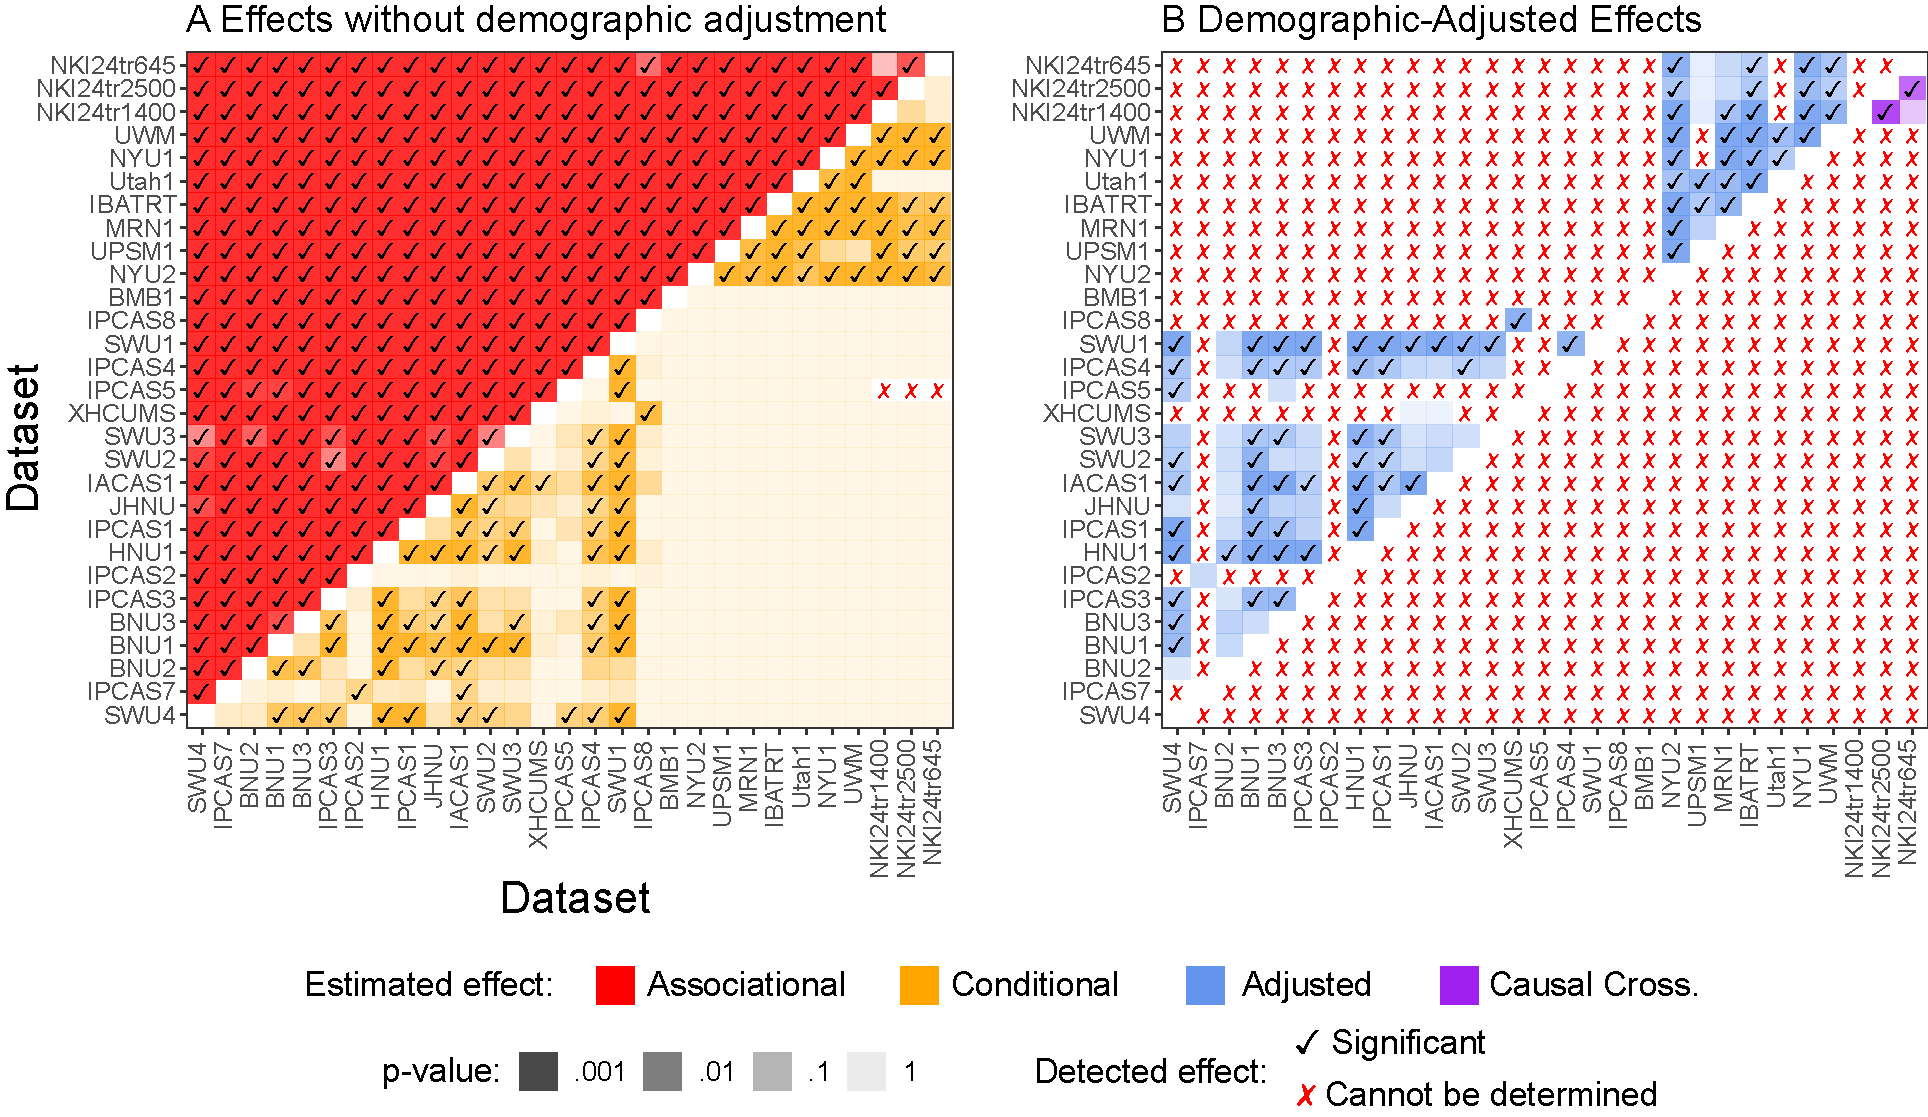
\includegraphics[width=\linewidth]{Figures/Content/raw_pairwise.pdf}
    \caption{\textbf{Comparison of Estimated Effects for CoRR Mega-Study}. Heatmaps indicating the $p$-value of effect estimates per pair of studies. Studies are organized by continent, followed by the number of samples in the study. Comparisons which are significant at $\alpha=.05$ are indicated by a black check. Since effects are symmetric (an effect between batch $t$ and $t'$ is equivalent to an effect between batch $t'$ and $t$), we collapse symmetric heatmaps into a single triangle for each effect type. \textbf{(A)} Effects which can be estimated but do not make direct adjustments for demographics. Associational and conditional effects can almost always be estimated between pairs of studies, so long as they share overlap in at least one covariate (IPCAS5 and NKI24 studies are entirely male or entirely female, entirely different continents, and entirely different age distributions, respectively, red Xs). \textbf{(B)} Effects which adjust for demographics through covariate adjustment. Squares in which an effect was not estimable due to covariate misalignment are indicated by a red X. Effects which adjust for demographics require covariate overlap across all covariates, which is indicated in Figure \ref{fig:demographic}B. A direct comparison of Figure \ref{fig:demographic}B between the conditional and adjusted procedures reveal that whereas conditional procedures tend to ``fail to reject'' with low or zero covariate overlap, adjusted procedures tend to avoid inference entirely.
    }
    \label{fig:raw_pairwise}
\end{figure}

Figure \ref{fig:raw_pairwise}A explores the four effects defined above in fMRI connectomes from the CoRR mega-study. {\edits{The majority of associational effects (99.8$\%$) are significant (distance correlation two-sample test, BH correction, $\alpha=0.05$). When we account for demographic covariates using conditional approaches, this drops to 25.8\% (conditional distance correlation two-sample test, BH correction, $\alpha=0.05$). Conceptually, both of these approaches are overly simplistic for concluding that a causal batch effect is indeed present because they fail to account for non-overlap of the covariate distributions between the subjects. In statistics, this is known as a ``fail to reject''; statistical inference via the conditional approach simply indicates to us that there is no evidence to reject the null hypothesis, and does not provide evidence for the null hypothesis (there is no effect). However, many of these comparisons are simply unreasonable to make in the first place.}}

Effects that account for demographic distributions are examined in Figure \ref{fig:raw_pairwise}B. Many pairs of studies could not have an adjusted effect estimated due to poor demographic alignment as shown in Figure \ref{fig:demographic}B, which resulted in no suitable matches existing between the studies, indicated by a red X ($279$ of $406$ pairs of studies). \textcolor{black}{Colloquially, when covariate overlap is moderate or limited as in Figure \ref{fig:sim_nlin_adjust}, we cannot tell if effects are misrepresented (or, comparisons are unreasonable entirely) due to demographic imbalance. In this way, causal strategies pre-pended to batch effect detection and mitigation strategies are \textit{more conservative in their application}, in that they prevent the experimenter from potentially deriving spurious or erroneous conclusions due to confounding biases, and directly indicate when comparisons are unreasonable to make}. Notably, adjusted conditional effects are estimable between all pairs of the American Clique (a group of separate studies consisting of similar demographics collected in North America, consisting of NYU1, NYU2, IBATRT, UWM, MRN1). After adjustment for the sample characteristics of the demographics associated with individual studies, a majority of adjusted effects (67.8$\%$) remain significant (causal conditional distance correlation two-sample test, BH correction, $\alpha=0.05$). 

The NKI Rockland Sample takes this a step further, allowing a crossover effect to be determined in a few pairs of batches (purple squares). This study was, in fact, collected on an identical set of participants, in the same location, with the same research technicians, with data varying only in the repetition time for the magnet used in the scanner. Indeed, for two of three comparisons, crossover effects remain prominent. This provides evidence that the parameters under which a study are conducted is a causal predictor of measured connectomes, assuming no participant state confounders are present.

% Word site effect => effect, but be clear we mean the effects discussed in 2.1
\label{sec:study_est_adjustment}

\subsection{Traditional Approaches Produce Disparate Inference from Techniques which Leverage Causality}
\textcolor{black}{At this point, we have demonstrated, through simulation and real examples, if a covariate is a \textit{confounder}, failure to properly account for demographic balancing can, potentially, yield improper detection and mitigation of batch effects and may, in turn, fundamentally alter true signals in the dataset. We saw that, for many of the CoRR \cite{corr} datasets, demographic balance was extremely poorly aligned, which allows only a fraction of the original possible comparisons between datasets to be analyzed in a theoretically, and empirically, reasonable manner. The final question we have is: does it matter? Even if we disrupt true signal in the dataset, can we still detect it irrespective of whether the signal is maintained in its unadulterated form?}

\textcolor{black}{To this end}, we investigate the strength of the sex effect, conditional on age, in the connectomes before and after batch effect correction (Figure \ref{fig:different}A). \Combat~and \cCombat~are performed on the entire CoRR study (top row) with age and sex covariates, and subsequently all techniques are restricted to the subset of connectomes upon which \cccombat~was executed (the \textit{American Clique}, bottom row). This amounts to the individuals within the study who were retained after matching on the basis of age, sex, and continent within the American Clique. We also compared these techniques to NeuroComBat (Conditional and Causal NeuroH) \cite{Fortin2018Feb,Pomponio2020Mar}, an implementation of \Combat~for neuroimaging data. The edges which show a significant, conditional sex effect (partial distance correlation, BH correction, $\alpha=.05$) are colored from smallest test statistic to largest test statistic (rank = 1, dark purple), and edges without a significant conditional sex effect are colored white. Causal approaches produce vastly different statistical inference compared to other correction techniques on the American Clique. Causal approaches were unable to be executed on the set of all studies, because many of the studies in the CoRR dataset do not overlap in terms of their covariate distributions (the red square indicates the analysis is not possible on the basis of continent, age, and sex). Next, we seek to answer whether statistical inference for the entire CoRR study (top row) is similar to inference that would be obtained on the American Clique (Figure \ref{fig:different}B) using only \cccombat. We compare the DICE overlap of the top $n$ edges (by effect size) from each of the three non-causal approaches applied to all the data with the top $n$ edges of \cccombat~on the American Clique. A high DICE overlap indicates that the subsets of edges are similar.  None of the techniques show high overlap with the edges that are indicated to have a large effect after correction with \cccombat. Finally, using the raw connectomes, \Combat, Conditional NeuroH, and \ccombat~tend to produce similar inferences, as all have high DICE overlaps near one.  In contrast, they all have low overlap with \cccombat~(Figure \ref{fig:different}C), with DICE overlap with \cccombat~nearly zero. On the other hand, Causal NeuroH has a high overlap with \cccombat. 
% The pairwise DICE overlaps are very similar regardless of which technique is used (DICE near $1$), whereas the DICE overlap with \cccombat~is extremely low (DICE near $0$).

\begin{figure}[h!]
    \centering
    \includegraphics[width=\linewidth]{Figures/Content/fig_dice.pdf}
    \caption{\textbf{Significant Edges Before and After Batch Effect Removal}. \textbf{(A)} The presence of a sex effect (conditional on individual age) is investigated for each edge in the connectome. The top 100 significant edges are shown in rank-order from largest (rank = 1) to smallest sex effect ($\alpha = .05$, Benjamini Hochberg \cite{BH} correction). Analysis is either performed over \textit{all} individuals (top row) or only upon the individuals for which sufficient demographic overlap could be obtained, the \textit{American clique} (bottom row). \cccombat~and Causal NeuroH can only be executed on the American Clique (red square denotes Causal approaches are not possible with \textit{all} studies). \textbf{(B)} The DICE overlap of the top $n$ edges of each batch effect removal technique on all the data (green squares, top row) as compared to those from \cccombat~(green square, bottom row). The red line (random) indicates the overlap to be obtained for a particular choice of $n$ to be expected as a result of random chance, and the gray ribbon indicates the 99\% confidence interval of the estimate ($1000$ repetitions). The DICE overlap increases as a function of $n$, regardless of whether any signal is actually present. \textbf{(C)} The DICE overlap of the top $100$ edges for all pairs of correction techniques indicated with a green square from \textbf{(A)}. Overlap of the top signal edges is high between no correction (raw), \Combat, \ccombat, and Conditional NeuroH, but all techniques have low overlap with \cccombat~and Causal NeuroH, indicating that Causal approaches yield measurements with signal that the associational approaches fail to identify.}
    \label{fig:different}
\end{figure}

% differences of effect sizes? what happens with effect sizes?
% DICE(top 100) raw, combat, conditional, neuroH vs causal cb, causal neuroHa

%
\clearpage
\section{Discussion}

Our primary conceptual contribution is establishing that batch effects can be formalized as causal effects.  Given this realization, we propose a framework for quantifying and removing batch effects in high-dimensional datasets featuring non-Euclidean measurements. We propose a straightforward approach to augment existing strategies for proper batch effect correction and removal, by first prepending existing techniques using causal balancing procedures. We explore the advantages of these procedures by demonstrating that causal approaches (such as \cccombat~and Causal \Dcorr) yield empirically valid approaches to handling batch effects, or report that no inference can be made. This represents a much more principled approach to alternative strategies which simply introduce or presume potentially disastrous artifactual biases. Finally, our neuroimaging use-case shows the utility of the methods developed herein for estimating and removing batch-related effects from large biological datasets. Specifically, our methods identify different causal effects as compared to prior approaches, each of which identifies features similar to a completely unadjusted approach, which are well established in the causal literature to permit numerous false positives and false negatives \cite{Ding2015Mar,Forstmeier2017Nov}. 
Together, our work rigorously defines and studies measurement bias decoupled from demographic confounders in complex, non-Euclidean data.

% In particular, when demographic overlap is enforced \textit{pre hoc} as with \cccombat~(i.e., enforcing demographic overlap prior to the removal of batch effects), we obtain a substantially different answer than when demographic overlap is enforced \textit{post hoc} after the application of competing batch effect correction methods. 
% % what I want to say: Figure 5A top row: we still get a different answer with other stuff
% When we did not enforce demographic overlap \textit{at all} for statistical inference, we still obtain a much different conclusion with both \ccombat~and \Combat~compared to \cccombat.

Together, the conclusions of our work bring into focus the pervasive question of how to properly interpret neuroimaging---or more generally, multi-site scientific---studies.%call into question how the conclusions of neuroimaging mega-studies apply outside of the particular subset of individuals upon which the analysis is performed. 
This concern is at the root of any statistical inference task: a conflict between the internal and external validity. Internal validity refers to how well the conclusions  generalize from the \textit{sample} population to the \textit{study} population; that is, from the observed samples to other samples that are distributed the same as the observed samples.
% the assumed set of individuals from which the \textit{sample} (the individuals who are analyzed during the investigation) is selected. 
External validity refers to the degree to which the conclusions generalize to the \textit{target} population; that is, the population to which we wish to apply the conclusions of our inferences. The target population is typically much broader than the study population, to include, for example, all members of the species, or possibly even multiple species. 

Through simulation, we demonstrated that minor misspecifications of the statistical model employed for batch effect removal can be disastrous in the presence of confounding. Specifically, a minor change of the relationship between the confounder (the covariate) and the measurement from a straight line to a (still monotonic) nonlinearity, the sigmoid, not only inhibited \ccombat~from removing a batch effect, but also introduced an artifact that dwarfed the magnitude of the original batch effect itself. As discussed in the Appendix \ref{app:sim_batch_adj} and expanded on via further simulations, the resulting estimate of the batch effect must, by construction, be considered neither statistically unbiased nor consistent, thus failing two preconditions for internal validity \cite{Westreich2019Feb}. Colloquially, it is almost impossible to know whether models employed for batch effect correction will be reasonable to apply to out-of-sample data (e.g., areas of the covariate distribution for which there is no covariate overlap). That is, we cannot tell whether the data we have will fall into Appendix Figure \ref{fig:sim_lin_adjust} or Appendix Figure \ref{fig:sim_nlin_adjust_nm_sym} and the batch effect correction technique will work reasonably given the underlying true signal, or Figure \ref{fig:sim_nlin_adjust}, Appendix Figure \ref{fig:sim_nlin_adjust_nm_asy}, or Appendix Figure \ref{fig:sim_nlin_adjust_nm_sym_asy} where the assumptions of the batch effect correction technique will be entirely unreasonable. On the other hand, causal strategies can help us to apply far more conservative logic, indicating to us when batch effects are unreasonable to estimate as is often the case with limited overlap in our simulations. Alternatively, they can aid us to first balance the covariate distributions so that we can avoid the pitfalls of the simulations which illustrate poor performance by \ccombat~in moderate or limited overlap regimes. Stated another way, in the absence of knowledge as to the appropriateness of the model employed for batch effect corrections, causal strategies make fewer assumptions about the covariate/outcome relationship to produce reasonable estimates.

Given the major shortcomings theoretically and empirically of traditional approaches for detecting and mitigating batch effects, we therefore chose to first prioritize the development of strategies which sub-sample individuals into demographically-aligned subsets using causal techniques. In so doing, we prioritized internal over external validity, as internal validity is a prerequisite for external validity. Colloquially, one cannot generalize results of an experiment to a target population if the results are, at best, dubiously applicable to the study population. The trade-off of subsampling individuals is that sample size, sample diversity, and  external validity are exchanged for internal validity. We saw this tradeoff materialize dramatically in the CoRR dataset, where over half of all possible dataset pairs could not be assessed for batch effects due to a lack of demographic alignment. This led to a much higher failure to reject rate in the conditional strategy than the adjusted causal strategy for batch effect detection.

The final hurdle of our analysis, therefore, is to address the question: does the internal validity of batch effect removal techniques actually impact downstream statistical inference? A failure to remove batch effects in an internally valid manner, we believe, presents a substantial hurdle for producing internally valid statistical inference downstream, since downstream statistical inference is a product of the corrected measurements. Specifically, one can  endeavor to mitigate batch effects in one of two complementary ways. First, one can filter individuals by ensuring demographic balancing, and then run the entire analysis only on those individuals (as causal approaches, like \cccombat~or Causal NeuroH, do).  Second, one can run an algorithm for batch effect correction (and potentially benefit from a richer number of samples), and then filter to ensure demographic balancing only when measuring downstream demographic-specific effect sizes (as we did by looking for a sex effect only considering individuals from the Raw, \Combat, \ccombat, and Conditional NeuroH~corrected connectomes in the American Clique). If internally valid, causal batch effect correction techniques may substantially restrict the sample size. Perhaps, even if the batch effect correction technique is not internally valid, measurements corrected using it may still have utility for downstream analysis. We anticipated that the most significant features for the inference task would be, at least, ordered similarly between the two analyses. However, our finding that the analyses produce radically different downstream inferences, even when we restrict the non-causal techniques to the same datasets, suggests that there is a link between downstream conclusions and the internal validity of batch effect correction techniques. Stated another way, when we perform batch correction using as few assumptions as possible about the study population through causal techniques, we get extremely disparate downstream scientific conclusions from state-of-the-art conditional techniques. 
This suggests to us that further work is needed to better understand how the removal of batch effects can be achieved while mitigating the deleterious effects on either internal or external validity through careful consideration of the study populations of analyses.

\paragraph*{Limitations and Future Work}

{\edits{The most prominent limitation of our work is that it appears as though we argue in favor of using strategies such as matching to pre-align measurements in terms of the covariate distributions. Indeed, this assumption is extremely restrictive: data will, inevitably, be discarded in the pursuit of internally reasonable estimates. Other techniques we could have leveraged, such as inverse propensity reweighting \cite{Stuart2010Feb}, subvert this limitation, but introduce the related issue that we are still estimating batch effects by upweighting or downweighting particular samples from the data. On the contrary, we do not advocate that the techniques proposed are the \textit{best} approaches one could use for batch effect correction. We posit that the techniques (e.g., prepending matching) or variations thereof (e.g., via inverse propensity reweighting) represent the only context in which naive \Combat, \ccombat, or related strategies leveraging potentially misspecified linear models could be applicable without rigorous justification of linear modeling choices in high-dimensional datasets with non-overlapping covariates as are often encountered in multi-site or multi-experiment mega-studies.

This limitation can be subverted by the development of more robust approaches for estimating the covariate/outcome relationship, building off the NeuroHarmonize approach \cite{Pomponio2020Mar} of incorporating non-linear modeling approaches (such as Generalized Additive Models, or GAMs) into the estimation process. With robust techniques to non-linearities for estimating the covariate/outcome relationship, the restrictive assumption of alignment of the propensity distributions can be exchanged with overlap of the propensity distributions, which informally means that the datasets must have a similar ``range'' of covariates (though, their distributions may differ, which is more realistic for observational data) \cite{Lopez2014}. Informally, you can ``guess'' the covariate/outcome relationship incorrectly and obtain reasonable estimates of batch effects as long as the covariate distributions are smiliar, or you can ``guess'' (or estimate) it correctly and need only covariates to be sufficiently represented in each batch. Unfortunately, estimating non-linear effects in high-dimensionality, low sample-size data (such as neuroimaging connectomes) has proven difficult, and most techniques approach this problem with an assumption of sparsity in the data \cite{Meier2009Dec,Huang2010Aug}, whereas the connectomes of this application (and numerous others, such as in genomics) are often dense. Strategies which can reasonably (explicitly or implicitly) estimate the covariate/outcome relationship provide an exciting avenue for future work.}
%In natively graph-valued data, we may be able to subvert the high-dimensionality, low sample-size problem by better understanding latent representations of the data that are simpler and less complicated. This may be accomplished via spectral methods \cite{Athreya2017Jan,Arroyo2021} or graph neural networks \cite{Xu2020Dec,Fu2020Feb}, in which batch effects could be studied and removed via a sparser representation of the graph data structure.}

Biomedical data science, including neuroimaging and connectomics, are plagued by a lack of generalizability and replicability \cite{Bridgeford2020Dec,Turner2018Jun}. Many investigations posit that this may be a consequence of small sample sizes or overly simplistic datasets \cite{Turner2018Jun,Nee2019Apr} lacking sufficient subject-specific measurements. We argue here that a lack of understanding regarding batch effects, and more fundamentally \textit{causality}, further exacerbates these issues. Indeed, these two perspectives may be considered complementary, in that with insufficient subject-specific measurements both causal and non-causal techniques will run into unmeasured confounding biases. \edits{A limitation of our proposed methods are that their adequacy to overcome confounding pre-supposes the measurement of a rich set of subject-specific covariates, which may often not be the case (and, likely, is not in the CoRR mega study). In this way, our real data investigation serves as illustrative of the wide disparities that can be found when leveraging causal techniques. On the other hand, with sufficient subject-specific covariates (e.g., more than age, biological sex, and continent as a loose proxy for race and culture) we are still likely to run into confounding issues which can be ameliorated by causal techniques such as those proposed herein.}

% what I want to say: Figure 5A bottom row: we get a different answer with causal combat than other stuff
% in this study, we chose to preserve internal over external validity
% We believe the tools and techniques devised in this work will prove critical to achieving these future aims.

%Across the experiments, we tend to find that $Z$-scoring and \Combat\ approaches tend to provide value eliminating disparate undesirable signal from connectomes. We tend to find that all strategies preserve some degree of biological variability in functional connectomes, when the biological variability is known ahead of time. This is evinced by the fact that both \Combat\ and $Z$-scoring show nearly identical detectability of demographic effects before and after correction for batch. What remains an open question, however, is how to best eliminate batch effects in isolation rather than simply removing all site effects (both batch effects and dmeographic effects). Both $Z$-scoring and \Combat\ eliminate all associational batch variability between datasets, even when such variability \textit{should} be present or desirable. For instance, a comparison of the Utah 1 dataset, a dataset containing only a single sex, to any other study indicates no between-batch variability, which is undesirable in cases where two datasets share vastly different demographic characteristics. This suggests that \textit{real biological variability} is being removed by naive \Combat\ correction, which is not ideal for pooled inference. On the other hand, \cccombat\ has preserved a substantial number of adjusted site effects, which also may not necessarily be desirable. It is important to highlight that \Combat\ assumes the data are vector-valued, and does not take careful consideration of the network topology of a connectome. This means that higher-order demographic effects (measured or unmeasured) may persist in the connectomes after removal of site effects. Strategies which adjust the network topology or properties related to the network topology (such as the \textit{latent positions} of a graph \cite{Chung2020Aug}), rather than the edge weights directly, may be more suitable for batch effect removal in connectomes. Future investigations may explore the trade-offs afforded by \Combat\ and novel strategies tailor designed for network-valued data for removing batch or batch effects in connectomics data.

To subvert this limitation, this work suggests that harmonized analyses should be conducted with both harmonized measurement parameters \textit{and} demographic distributions. This represents a departure from the manner in which many mega-studies, including so-called harmonized effects, are currently generated \cite{corr,di2014autism,di2017enhancing,Yamashita2019Apr}, in which potentially demographically-disparate populations are analyzed and only loosely harmonized on the basis of the measurement protocols. We saw that post-hoc batch effect detection and removal (and consequently, downstream statistical inference) presents both theoretical and conceptual inconsistencies with regard to internal validity when not first passed through the lens of causality. {\edits{This problem is highlighted by looking at the poor demographic overlap for popular neuroimaging studies such as CoRR in Figure \ref{fig:demographic}, and in the ABIDE study \cite{di2014autism,di2017enhancing} detailed in Appendix Figure \ref{fig:overlap2}. While the SRBPS \cite{Yamashita2019Apr} has greater overlap on the basis of age, sex, and likely race (same continent) for many pairs of datasets (but still has two datasets that are dissimilar from the others), both ABIDE and SRBPS add the additional hurdle of neurodivergences being used in participant recruitment to batches. If the connectome is a proxy for brain function, neurodivergent brain features captured by the connectome may cause symptoms of neurodivergence \cite{Vogelstein2019Apr,Konrad2010Jun,Hashem2020}, introducing a potential causal mediation effect if the neurodivergence is leveraged directly in participant recruitment \cite{Pearl2014Dec,Bareinboim2012Mar}. While this issue has been explored for the wider problem of data fusion \cite{Bareinboim2016Jul}, is unclear the extent to which causal mediation impacts batch effect detection or correction in high-dimensional biological studies.}}

Future work will focus on applying the methods developed here to harmonize mega-studies such as the Adolescent Brain Cognitive Development (ABCD) \cite{Karcher2021Jan}, which includes $N>12,000$ demographically diverse individuals from across the United States, and measurements were produced with a consistent, harmonized measurement protocol. Further, future studies may seek to build upon the NKI-RS and the recent work by \citet{Noble2017Feb} by collecting measurements from the same expansive and diverse group of people across multiple neuroimaging sites or scanning protocols. Our work provides a theoretical foundation for evaluating existing neuroimaging studies, such as \citet{Noble2017Feb} and \cite{Yamashita2019Apr}, which advocate for the aggregation of studies featuring individuals measured at a wide array of sites (so called \textit{travelling subject} datasets), so that the nature of batch effects can be explored with minimal assumptions needed due to the crossover property. In such datasets, scientists can appreciate internally valid demographic-specific effects on the measurement, and learn more reasonable modeling assumptions, so that perhaps extrapolatory pre- or post-hoc batch effect removal techniques (such as in Appendix Figure \ref{fig:sim_lin_adjust}) can be employed to mitigate the batch effects in other non-demographic-aligned datasets. Failure to attain a comprehensive understanding of batch effects and the extent to which they pervade statistical inferences, we believe, calls into question the validity of existing results in scientific meta-analyses. 

\section*{Code Availability}

The code used for analysis within this manuscript is available at \\ \href{https://github.com/ebridge2/batch_effects}{github.com/ebridge2/batch\_effects}, and a docker container with all software versions is available at \href{https://hub.docker.com/r/neurodata/batch_effects}{hub.docker.com/r/neurodata/batch\_effects}.

\section*{Data Availability}

The raw data analyzed in this manuscript can be obtained at \href{http://fcon_1000.projects.nitrc.org/indi/CoRR/html/}{CoRR Mega-Study}. The pre-processed data analyzed in this manuscript is available at \href{https://neurodata.io/mri/}{neurodata.io/mri}.

\section*{Contributions}

EWB wrote the manuscript; EWB and JTV revised the manuscript; EWB, JTV, and MP conducted study conception and design; EWB, JTV, BC, and MP conducted interpretation of results; EWB, JC, SP, and RL analyzed raw neuroimaging and demographic data; EWB and JTV devised the statistical methods; EWB analyzed processed data; MP, GK, SN, TX, MM, BC, and JTV provided valuable feedback and discussion throughout the work.

\subsection*{Acknowledgements}
% UPenn, NSF Career Award, Duke
% add Stephanie, Betsy
The authors are grateful for the support from the National Science Foundation (NSF) administered through NSF Career Award NSF 17-537, the National Institute of Health (NIH) through National Institute of Mental Health (NIMH) Research Project 1R01MH120482-01, and the NIH through Research Project RO1AG066184-01. We also wanted to thank Betsy Ogburn for numerous insightful conversations regarding the presentation and framing of this work. 
% TODO@jv: who is duke PI?

% \section{Methods (Expanded)}

\label{sec:notnovel_methods}

\subsection{Covariate Adjustment}
\label{sec:covar_adjustment}
The exposed group $t$ is selected to be the smaller of the two groups, and the unexposed group $t'$ is selected to be the larger of the two groups, where $n_t$ is the number of individuals in the exposed group and $n_{t'}$ is the number of individuals in the unexposed group. The ``covariate overlap'' procedure attempts to ensure positivity of the propensity distribution for the unexposed group (i.e., $e(t'|x) > 0$). Intuitively, we exclude individuals from the unexposed group who do not appear ``similar'' to individuals in the exposed group. In this work, covariate overlap is established through logistic regression by excluding individuals in the control group with a propensity for exposure lower than $0.01$. Similarly, the ``covariate balancing'' procedure attempts to re-weight observations in the per-batch covariate distributions such that the covariate distributions are approximately equal (i.e., $f(x|t) \approx f(x|t')$). In this work, we perform $k:1$ nearest-neighbor matching using the \texttt{MatchIt} package \cite{matchit}. The number of matches $k = \floor{\frac{n_{t'}}{n_t}}$ is chosen to be the largest number of unexposed matches possible. Individuals are balanced on the basis of individual sex, individual age, and continent of study. As there are likely many other categories with which brain connectivity may be confounded, we do not believe this covariate set is necessarily sufficient to identify a Causal Batch Effect \ref{def:causal_batch_informal}, as we would need to be confident that these covariates exhibited the covariate sufficiency property. We perform exact matching on the basis of individual sex and individual continent of measurement, and use a $0.1$-standard deviation caliper on the propensity score to obtain at most $k$ matched participants for each treated individual \cite{Powell2020Sep}.

\subsection{Hypothesis Testing}

\label{app:hypo_testing}
Recall that statements of the form $f(y) = g(y)$ against $f(y) \neq g(y)$ are equivalent to $P_f = P_g$ against $P_f \neq P_g$, as probability densities uniquely define distribution functions. Therefore, hypotheses for the effects described in Section \ref{sec:methods} require two-sample and conditional two-sample testing procedures. A natural test statistic for the two-sample testing procedure is the Distance Correlation \cite{Szekely2007Dec}, which is a non-parametric test for testing whether two variables are correlated. A simple augmentation of the distance correlation procedure \cite{Shen2017-ub,Vogelstein2019-zt} shows that \texttt{DCorr} can be used for the two-sample test, or a test of whether two samples are drawn from different distributions. \texttt{DCorr} is exactly equivalent in this context to the Maximum Mean Discrepency (MMD), which embeds points in a reproducing kernel Hilbert Space (RKHS) and looks for functions over the unit ball in the RKHS that maximize the difference of the means of the embedded points. When we instead consider the conditional two-sample test (i.e., a test of $f(y|x)= g(y|x)$ against $f(y|x) \neq g(y|x)$), we instead use the conditional distance correlation \cite{Wang2015}, a kernel-based approach in which the points are embedded in a new, non-linear Hilbert Space, which augments the traditional linear Hilbert Space used in distance correlation to allow the definition of the squared distance covariance. Below, we let $\mathbf Y = (y_i) \in \mathcal Y^n$ denote realizations across both samples and $\vec t = (t_i) \in \{t, t'\}^n$ indicate from which sample each realization is drawn. $\mathbf X = (x_i) \in \mathcal X^n$ denotes covariates which are known about the objects of interest.

\paragraph{Associational Effect}

We have the following null and alternative hypotheses:
\begin{align*}
    H_0 : f(y|t) = f(y|t')\text{ against }H_A: f(y|t) \neq f(y|t')
\end{align*}
A test of the preceding hypotheses is performed using the distance correlation, and the natural test statistic is $\texttt{DCorr}(\mathbf Y, \vec t)$.

\paragraph{Conditional Effect}

We have the following null and alternative hypotheses:
\begin{align*}
    H_0: f(y|t,x) = f(y|t',x) \text{ against }H_A: f(y|t,x) \neq f(y|t',x)
\end{align*}
A test of the preceding hypotheses is performed using the conditional distance correlation, and the natural test statistic is $\texttt{cDCorr}(\mathbf Y, \vec t | \mathbf X)$. 

\paragraph{Adjusted Conditional Effect}

We have the following null and alternative hypotheses:
\begin{align*}
    H_0: \tilde f(y|t,x) = \tilde f(y|t',x) \text{ against }H_A: \tilde f(y|t,x) \neq \tilde f(y|t',x)
\end{align*}
Unlike the preceding tests, we instead consider the data $(\tilde {\mathbf Y}, \vec{\tilde t}, \tilde {\mathbf X})$, which are the measurements, sample indicators, and covariates of the $n$ realizations after covariate adjustment. A test of the preceding hypotheses is performed using the conditional distance correlation, and the natural test statistic is $\texttt{cDCorr}(\mathbf {\tilde Y}, \vec {\tilde t} | \mathbf {\tilde X})$. 

\paragraph{Causal Crossover Effect}

We have the following null and alternative hypotheses:
\begin{align*}
    H_0: f\parens*{y^{(t)} \big | t, x^{(t)}} = f\parens*{y^{(t')} \big | t', x^{(t')}}\text{ against }H_A: H_0: f\parens*{y^{(t)} \big | t, x^{(t)}} \neq f\parens*{y^{(t')} \big | t', x^{(t')}}
\end{align*}
If the known covariates are identical between batches $t$ and $t'$, we test the preceding hypotheses using the distance correlation, and the natural test statistic is $\texttt{DCorr}(\mathbf Y, \vec t)$. If the known covariates are not identical between batches $t$ and $t'$, we test the preceding hypotheses using the conditional distance correlation, and the natural test statistic is $\texttt{cDCorr}(\mathbf Y, \vec t | \mathbf X)$.

\paragraph{More Than Two Batches}

The above approaches generalize sufficiently to $K$ batches using $K$-sample testing approaches \cite{Bridgeford2023Jul}. With $f_k$ for $k \in [K]$ denoting the densities associated with $K$ sites or batches, this motivates hypotheses of the form:
\begin{align*}
    H_0 : f_k = f_l \text{ for all }k, l \text{ against }H_A: f_k \neq f_l \text{ for some }k \neq l,
\end{align*}
which can be tested using the distance correlation or the conditional distance correlation as above, with the caveat that $\vec t$ becomes the matrix $\mathbf T = (t_{i,k}) \in \{0, 1\}^{n \times K}$. Each entry $t_{ik} = 1$ if sample $i$ is in batch $k$, and $0$ otherwise. For the purposes of this manuscript, we focus on the two-batch case.

\paragraph{$p$-values and Multiple Hypothesis Correction}

$p$-values in this manuscript are estimated using permutation testing, which is an approach to obtain the distribution of the test statistic under the null with minimal assumptions and approximations \cite{Efron2004Mar}. All $p$-values are estimated using $N=1$,$000$ (detection, Figure \ref{fig:raw_pairwise}) or $N=10$,$000$ (correction, Figure \ref{fig:different}) permutations. Across all figures associated with this work, we are concerned with obtaining a proper estimate of the rate at which we detect effects (\textit{discoveries}). Therefore, we control the false discovery rate (FDR) with the Benjamini-Hochberg Correction \cite{BH}. 



% The preceding effects motivate the the null hypothesis that the effect is not present against the alternative that the effect is present. For the associational effect and the causal crossover effect, we leverage the distance correlation (\texttt{DCorr}) \cite{Szekely2007Dec}, a kernel-based test statistic that is equivalent to the Maximum Mean Discrepancy (MMD) \cite{Shen2017-ub,Vogelstein2019-zt}. For the conditional effect and the adjusted effect, we leverage the partial distance corrlation (\texttt{cDCorr}) \cite{Szekely2014Dec}. $p$-values are estimated using permutation testing with $N=10,000$ permutations, and are adjusted using the Benjamini-Hochberg procedure \cite{BH}. Further details on hypothesis testing are found in Appendix \ref{app:hypo_testing}.


\subsection{Batch effect correction via $z$-scoring}

We compare $z$-scoring per-feature within each batch \cite{Lazar2013Jul} and traditional \Combat\ to Causal \Combat. For a given edge $y_{i}^{(t)}(k,l)$ $(k, l)$ for an individual $i$ in batch $t$, we define the $z$-score corrected edge-weight to be:
\begin{align*}
    z_{i}^{(t)}(k, l) = \frac{y_i^{(t)}(k, l) - \bar y^{(t)}(k, l)}{s^{(t)}(k, l)},
\end{align*}
where $\bar y^{(t)}(k, l)$ is the sample mean and $s^{(t)}(k, l)$ is the sample standard deviation for edge $(k, l)$ in batch $t$. These strategies reduce known topological properties of human connectomes; particularly, homotopy, as shown in Figure \ref{fig:top_hist} and Figure \ref{fig:site_individual} and are therefore not considered for more careful analysis.

\subsection{Control Numerical Experiments}

Control experiments are performed to ensure that after batch effect correction, the resulting data maintains interpretability and utility for scientific inquiry. Even if the data is devoid of batch effects, it must still be useful for downstream inference. For our connectome data, we identify two key control scenarios, the preservation of demographic effects and the preservation topological effects, which are desirable to preserve after batch effect correction.

\label{app:control}
\paragraph{Testing Topological Properties}


\paragraph{Demographic Effect}

Demographic effects are investigated across both the subset of connectomes upon which Causal \Combat~ is executed (the American Clique) and the full dataset. We observe the tuple $\parens*{y_{i}(k,l), s_i, a_i, t_i}$ for $i \in [n]$, and $k, l \in [V]$, where $V=116$ denotes the number of parcels in the Automated Anatomical Labelling (AAL) parcellation \cite{aal}. We suppose that $Y(k,l)$ is the $[0,1]$-valued random variable denoting the weight of edge $(k,l)$, $S$ is the binary-valued random variable denoting the biological sex, $A$ is the positive real-valued random variable denoting age, and $T$ is the $[K]$-valued random variable denoting the batch. We let $\vec y{(k,l)} = \parens*{y_{i}(k,l)} \in \mathcal [0,1]^n$ denote the realized edge weights, $\vec s = (s_i) \in \{0,1\}^n$ denote the realized biological sexes, $\vec a = (a_i) \in \realn^n$ denote the realized biological ages, and $\vec t = (t_i) \in [K]^n$ denote the realized batches. We say that a \textbf{demographic sex effect} exists when:
\begin{align*}
    f(y | a, s) \neq f(y|a,s')
\end{align*}
To test for a demographic sex effect, we have the following null and alternative hypotheses:
\begin{align*}
    H_0: f(y | a, s) = f(y | a, s') \text{ against }f(y|a,s) \neq f(y|a,s')
\end{align*}
We are able to test the preceding hypothesis using the partial distance correlation, and the test statistic is $\texttt{pDCorr}(\vec y(k,l), \vec s | \vec a)$.

% \paragraph{Demographic Effect}

% Demographic effects are investigated within each batch separately, to \textit{eliminate} the possible confounding of unobserved demographic and batch effects. Within a single batch $t$, We observe the tuple $(y_i, s_{i}, a_{i})$, for $i \in [n_t]$. We suppose that $S$ is the binary-valued random variable denoting the biological sex, and $A$ is the positive real valued random variable denoting age. We let $\mathbf Y = (y_i) \in \mathcal Y^{n_t}$ denote the realized measurements, $\vec s = (s_i) \in \{0,1\}^{n_t}$ denotes the realized biological sexes, and $\vec a = (a_i) \in \realn_+^{n_t}$ denotes the realized ages.

% We define that a \textbf{demographic age effect} exists when:
% \begin{align*}
%     f(y|a, s) \neq f(y|a', s)
% \end{align*}
% To test for a demographic age effect, we have the following null and alternative hypotheses:
% \begin{align*}
%     H_0: f(y|a, s) = f(y|a', s) \text{ against }H_A: f(y|a, s) \neq f(y|a', s)
% \end{align*}
% We test the preceding hypotheses using the partial distance correlation, and the test statistic is $\texttt{cDCorr}(\mathbf Y, \vec a | \vec s)$. 

% Similarly, we define that a \textbf{demographic sex effect} exists when:
% \begin{align*}
%     f(y|a, s) \neq f(y|a, s')
% \end{align*}
% Where $s \neq s'$.

% To test for a demographic sex effect, we have the following null and alternative hypotheses:
% \begin{align*}
%     H_0: f(y|a, s) = f(y|a, s') \text{ against }H_A: f(y|a, s) \neq f(y|a, s')
% \end{align*}
% We test the preceding hypotheses using the partial distance correlation, and the test statistic is $\texttt{cDCorr}(\mathbf Y, \vec s | \vec a)$. 



\subsection{Datasets}
\label{sec:corr_descr}
The CoRR Mega-Study \cite{corr} is an aggregate dataset consisting of $27$ studies collected with a similar goal: assessing the reliability and reproducibility of neuroimaging data. The mega-study consists of $1313$ individuals, most of whom are measured numerous times, for a total of $N=3597$ connectomes. All connectomes are estimated using the \texttt{m2g} (MRI to Graphs) pipeline \cite{m2g}, which provides a wrapper for the \texttt{CPAC} Pipeline \cite{cpac}. fMRI scans for each individual are first processed to remove motion artifacts using \texttt{mcflirt} \cite{flirt}. The fMRI scans are then registered to the corresponding individual's anatomical scan using FSL's boundary-based registration (BBR) via \texttt{epireg} \cite{epireg}. A non-linear transformation from the individual's anatomical scan to the MNI152 \cite{mni152} template is estimtaed using \texttt{FNIRT} \cite{fnirt}. Nuisance artifacts are removed by fitting the voxelwise timeseries to a regression model incorporating regressors for the Friston 24-parameter model \cite{friston24}, the top five principal components of the voxelwise timeseries in cerebrospinal fluid \texttt{aCompCor} \cite{acompcor}, and a quadratic drift term. The adjusted voxelwise timeseries is downsampled to the regions of interest (ROIs) of the Automated Anatomical Labelling (AAL) parcellation \cite{aal} by taking the spatial mean signal for each timepoint across voxels within the region of interest. Functional connectivity is estimated using the pairwise correlation between all pairs of ROI timeseries within the AAL parcellation. Parcels are sorted throughout the manuscript according to hemispheric order, in which the parcels are aligned with left hemisphere parcels followed by right hemisphere parcels. Within hemisphere, parcels are sorted by AAL parcel number. For each study, we have baseline covariates for the continent, sex, and the age of participants.


\paragraph{The American Clique} The ``American Clique'' describes a subset of the CoRR Mega-Study in which the sample populations share similarities in sample demographic characteristics. These studies share a demographic focusing on males and females (in roughly equal proportions) of individuals across a wide age range, and include the ``NYU2'', ``IBATRT'', ``MRN1'', ``UWM'', and ``NYU1'' studies. The $833$ connectomes comprising the studies of the American clique are reduced to the $N=321$ connectomes with maximal demographic overlap identified through covariate adjustment \ref{sec:covar_adjustment}.

\paragraph{The NKI Rockland Sample} \cite{nkirs} is a single study from the CoRR Mega-Study consisting of 24 individuals, each of whom is measured two times across three functional MRI acquisition protocols, which vary in the repetition time for each slice of the sequence (TR). The data was collected with the intention of investigating the impact of the different MRI protocols in a crossover-randomized approach. Due to the crossover property, evidence in favor of an effect provides strong evidence of a causal batch effect. Images with a TR of 645 millisecond (ms), 1400 ms, and 2500 ms are measured, with the prompt for each subject remaining identical.





\bibliographystyle{plainnat}
\bibliography{batch}

\appendix

% \include{Appendix/methods_long}
\section{Procedures for detecting and mitigating batch effects}
\label{app:causal_procedures}

\subsection{Detecting batch effects with \ccdcorr}
Many of the more direct types of detectable effects, such as associational and conditional effects, fail to adaequately account for confounding biases present in the data. {\edits{We instead propose the use of \ccdcorr, in which a conditional $K$-sample test \cite{Wang2015} is performed on samples with the same ``range'' of covariate values after propensity trimming via a strategy known as vector matching \cite{Lopez2014}. This strategy is the focus of a complementary theoretical manuscript, in which we illustrate the theoretical and empirical (via simulations) benefits of this technique over competing approaches for detecting causal effects between potential outcomes. This strategy maintains both high sensitivity and specificity under traditionally problematic data regimes (high-dimensionality, non-monotonicities, and non-linearities) in which other methods typically fail \cite{Bridgeford2023Jul}, making it a natural choice for causal discrepancy testing (of which ``batch effect'' detection, termed \textit{causal unconditional discrepancy testing} in \cite{Bridgeford2023Jul}, as-defined herein is a special case).

{Figure \ref{fig:demographic}C illustrates visually the causal procedures employed for adjusting the batches}. Rather than fully matching to produce the adjusted batches, samples are retained only such that they have approximately overlapping covariate distributions (propensity trimming, shaded boxes). A full schematic illustrating the use of vector matching is detailed in Appendix E of \cite{Bridgeford2023Jul}. In the event that the batch assignment mechanism is ignorable given the covariates and that effects between datasets are in the same direction across all covariate levels, the adjusted effect detected by \ccdcorr~is a causal batch effect, as proven in \cite{Bridgeford2023Jul}. That the effects between datasets are in the same ``direction'' across all covariate levels can be best intuited via example. Consider the case where a batch effect exists, such that there is a signal disparity (a difference in the expected connectivity) in a particular edge of a connectome between two batches. If this signal disparity is a positive difference between batches $1$ and $2$ across all covariate levels (or, a negative difference across all covariate levels), \ccdcorr~will detect a causal batch effect. In the event that the assignment mechanism is ignorable but that effects between datasets are not in the same direction across all covariate levels, the adjusted effect detected by \ccdcorr~is a causal effect, but may reflect a \textit{causal conditional discrepancy} (e.g., there are batch-specific differences, but they are isolated to particular covariate levels). In the event that the batch assignment mechanism is not ignorable, the effect may not reflect any causal effects (e.g., it may reflect unmeasured demographic differences between the batches).}}


\subsection{Mitigating batch effects using Causal \Combat}

% \paragraph{Causal Combat}

Unfortunately, many existing techniques for the removal of batch effects fail to adequately account for confounding biases that may be present in the data. We propose Causal \Combat, in which Conditional \Combat\ is performed on a subset of observational studies in which all pairs of studies are balanced against measured demographic covariates.
% 
Causal \Combat\ is performed as follows. Given measurements and covariates from $n$ individuals across $K$ batches, each of which has $n_k$ individuals:
\begin{enumerate}[leftmargin=*]
    \item Identify the smallest dataset $k'$ as the exposure dataset and all $k \neq k'$ datasets as control datasets.
    \item Propensity trim and then match the greatest integer less than $n_k/n_{k'}$ control individuals using nearest-neighbor matching to individuals in the exposure dataset. Methods \ref{sec:notnovel_methods} discusses the adjustment procedure in more detail.
    \item Discard individuals from the exposure dataset who do not have matches in all $K$ control datasets, yielding the matched exposure cohort.
    \item Discard individuals from the control datasets who are not matched to the matched exposure cohort, yielding the matched control cohorts.
    \item Perform Conditional \Combat\ \cite{Johnson2007Jan} on the measurements of the matched exposure and matched control individuals across the $K$ batches, conditioned on the measured covariates $X$.
\end{enumerate}
In the event that the conditioning set closes backdoor paths \cite{Pearl2009Jan,Pearl2010Jul}, Causal \Combat\ yields the removal of an internally valid causal effect and does not require extrapolation assumptions, unlike Conditional \Combat\ \cite{Stuart2010Feb,matchit,Rosenbaum1983Apr,Rosenbaum1985}. If the conditioning set does not close backdoor paths, the effect removed is a conditional effect and may potentially yield the removal of demographic effects, as we saw in Figure \ref{fig:sim_nlin_adjust}. Appendix \ref{app:overlap} depicts the impact on the empirical covariate distribution of the adjustment procedure.

\section{Methods (Expanded)}

\label{sec:notnovel_methods}

\subsection{Covariate Adjustment}
\label{sec:covar_adjustment}
The exposed group $t$ is selected to be the smaller of the two groups, and the unexposed group $t'$ is selected to be the larger of the two groups, where $n_t$ is the number of individuals in the exposed group and $n_{t'}$ is the number of individuals in the unexposed group. The ``covariate overlap'' procedure attempts to ensure positivity of the propensity distribution for the unexposed group (i.e., $e(t'|x) > 0$). Intuitively, we exclude individuals from the unexposed group who do not appear ``similar'' to individuals in the exposed group. In this work, covariate overlap is established through logistic regression by excluding individuals in the control group with a propensity for exposure lower than $0.01$. Similarly, the ``covariate balancing'' procedure attempts to re-weight observations in the per-batch covariate distributions such that the covariate distributions are approximately equal (i.e., $f(x|t) \approx f(x|t')$). In this work, we perform $k:1$ nearest-neighbor matching using the \texttt{MatchIt} package \cite{matchit}. The number of matches $k = \floor{\frac{n_{t'}}{n_t}}$ is chosen to be the largest number of unexposed matches possible. Individuals are balanced on the basis of individual sex, individual age, and continent of study. As there are likely many other categories with which brain connectivity may be confounded, we do not believe this covariate set is necessarily sufficient to identify a Causal Batch Effect \ref{def:causal_batch_informal}, as we would need to be confident that these covariates exhibited the covariate sufficiency property. We perform exact matching on the basis of individual sex and individual continent of measurement, and use a $0.1$-standard deviation caliper on the propensity score to obtain at most $k$ matched participants for each treated individual \cite{Powell2020Sep}.

\subsection{Hypothesis Testing}

\label{app:hypo_testing}
Recall that statements of the form $f(y) = g(y)$ against $f(y) \neq g(y)$ are equivalent to $P_f = P_g$ against $P_f \neq P_g$, as probability densities uniquely define distribution functions. Therefore, hypotheses for the effects described in Section \ref{sec:methods} require two-sample and conditional two-sample testing procedures. A natural test statistic for the two-sample testing procedure is the Distance Correlation \cite{Szekely2007Dec}, which is a non-parametric test for testing whether two variables are correlated. A simple augmentation of the distance correlation procedure \cite{Shen2017-ub,Vogelstein2019-zt} shows that \texttt{DCorr} can be used for the two-sample test, or a test of whether two samples are drawn from different distributions. \texttt{DCorr} is exactly equivalent in this context to the Maximum Mean Discrepency (MMD), which embeds points in a reproducing kernel Hilbert Space (RKHS) and looks for functions over the unit ball in the RKHS that maximize the difference of the means of the embedded points. When we instead consider the conditional two-sample test (i.e., a test of $f(y|x)= g(y|x)$ against $f(y|x) \neq g(y|x)$), we instead use the conditional distance correlation \cite{Wang2015}, a kernel-based approach in which the points are embedded in a new, non-linear Hilbert Space, which augments the traditional linear Hilbert Space used in distance correlation to allow the definition of the squared distance covariance. Below, we let $\mathbf Y = (y_i) \in \mathcal Y^n$ denote realizations across both samples and $\vec t = (t_i) \in \{t, t'\}^n$ indicate from which sample each realization is drawn. $\mathbf X = (x_i) \in \mathcal X^n$ denotes covariates which are known about the objects of interest.

\paragraph{Associational Effect}

We have the following null and alternative hypotheses:
\begin{align*}
    H_0 : f(y|t) = f(y|t')\text{ against }H_A: f(y|t) \neq f(y|t')
\end{align*}
A test of the preceding hypotheses is performed using the distance correlation, and the natural test statistic is $\texttt{DCorr}(\mathbf Y, \vec t)$.

\paragraph{Conditional Effect}

We have the following null and alternative hypotheses:
\begin{align*}
    H_0: f(y|t,x) = f(y|t',x) \text{ against }H_A: f(y|t,x) \neq f(y|t',x)
\end{align*}
A test of the preceding hypotheses is performed using the conditional distance correlation, and the natural test statistic is $\texttt{cDCorr}(\mathbf Y, \vec t | \mathbf X)$. 

\paragraph{Adjusted Conditional Effect}

We have the following null and alternative hypotheses:
\begin{align*}
    H_0: \tilde f(y|t,x) = \tilde f(y|t',x) \text{ against }H_A: \tilde f(y|t,x) \neq \tilde f(y|t',x)
\end{align*}
Unlike the preceding tests, we instead consider the data $(\tilde {\mathbf Y}, \vec{\tilde t}, \tilde {\mathbf X})$, which are the measurements, sample indicators, and covariates of the $n$ realizations after covariate adjustment. A test of the preceding hypotheses is performed using the conditional distance correlation, and the natural test statistic is $\texttt{cDCorr}(\mathbf {\tilde Y}, \vec {\tilde t} | \mathbf {\tilde X})$. 

\paragraph{Causal Crossover Effect}

We have the following null and alternative hypotheses:
\begin{align*}
    H_0: f\parens*{y^{(t)} \big | t, x^{(t)}} = f\parens*{y^{(t')} \big | t', x^{(t')}}\text{ against }H_A: H_0: f\parens*{y^{(t)} \big | t, x^{(t)}} \neq f\parens*{y^{(t')} \big | t', x^{(t')}}
\end{align*}
If the known covariates are identical between batches $t$ and $t'$, we test the preceding hypotheses using the distance correlation, and the natural test statistic is $\texttt{DCorr}(\mathbf Y, \vec t)$. If the known covariates are not identical between batches $t$ and $t'$, we test the preceding hypotheses using the conditional distance correlation, and the natural test statistic is $\texttt{cDCorr}(\mathbf Y, \vec t | \mathbf X)$.

\paragraph{More Than Two Batches}

The above approaches generalize sufficiently to $K$ batches using $K$-sample testing approaches \cite{Bridgeford2023Jul}. With $f_k$ for $k \in [K]$ denoting the densities associated with $K$ sites or batches, this motivates hypotheses of the form:
\begin{align*}
    H_0 : f_k = f_l \text{ for all }k, l \text{ against }H_A: f_k \neq f_l \text{ for some }k \neq l,
\end{align*}
which can be tested using the distance correlation or the conditional distance correlation as above, with the caveat that $\vec t$ becomes the matrix $\mathbf T = (t_{i,k}) \in \{0, 1\}^{n \times K}$. Each entry $t_{ik} = 1$ if sample $i$ is in batch $k$, and $0$ otherwise. For the purposes of this manuscript, we focus on the two-batch case.

\paragraph{$p$-values and Multiple Hypothesis Correction}

$p$-values in this manuscript are estimated using permutation testing, which is an approach to obtain the distribution of the test statistic under the null with minimal assumptions and approximations \cite{Efron2004Mar}. All $p$-values are estimated using $N=1$,$000$ (detection, Figure \ref{fig:raw_pairwise}) or $N=10$,$000$ (correction, Figure \ref{fig:different}) permutations. Across all figures associated with this work, we are concerned with obtaining a proper estimate of the rate at which we detect effects (\textit{discoveries}). Therefore, we control the false discovery rate (FDR) with the Benjamini-Hochberg Correction \cite{BH}. 



% The preceding effects motivate the the null hypothesis that the effect is not present against the alternative that the effect is present. For the associational effect and the causal crossover effect, we leverage the distance correlation (\texttt{DCorr}) \cite{Szekely2007Dec}, a kernel-based test statistic that is equivalent to the Maximum Mean Discrepancy (MMD) \cite{Shen2017-ub,Vogelstein2019-zt}. For the conditional effect and the adjusted effect, we leverage the partial distance corrlation (\texttt{cDCorr}) \cite{Szekely2014Dec}. $p$-values are estimated using permutation testing with $N=10,000$ permutations, and are adjusted using the Benjamini-Hochberg procedure \cite{BH}. Further details on hypothesis testing are found in Appendix \ref{app:hypo_testing}.


\subsection{Batch effect correction via $z$-scoring}

We compare $z$-scoring per-feature within each batch \cite{Lazar2013Jul} and traditional \Combat\ to Causal \Combat. For a given edge $y_{i}^{(t)}(k,l)$ $(k, l)$ for an individual $i$ in batch $t$, we define the $z$-score corrected edge-weight to be:
\begin{align*}
    z_{i}^{(t)}(k, l) = \frac{y_i^{(t)}(k, l) - \bar y^{(t)}(k, l)}{s^{(t)}(k, l)},
\end{align*}
where $\bar y^{(t)}(k, l)$ is the sample mean and $s^{(t)}(k, l)$ is the sample standard deviation for edge $(k, l)$ in batch $t$. These strategies reduce known topological properties of human connectomes; particularly, homotopy, as shown in Figure \ref{fig:top_hist} and Figure \ref{fig:site_individual} and are therefore not considered for more careful analysis.

\subsection{Control Numerical Experiments}

Control experiments are performed to ensure that after batch effect correction, the resulting data maintains interpretability and utility for scientific inquiry. Even if the data is devoid of batch effects, it must still be useful for downstream inference. For our connectome data, we identify two key control scenarios, the preservation of demographic effects and the preservation topological effects, which are desirable to preserve after batch effect correction.

\label{app:control}
\paragraph{Testing Topological Properties}


\paragraph{Demographic Effect}

Demographic effects are investigated across both the subset of connectomes upon which Causal \Combat~ is executed (the American Clique) and the full dataset. We observe the tuple $\parens*{y_{i}(k,l), s_i, a_i, t_i}$ for $i \in [n]$, and $k, l \in [V]$, where $V=116$ denotes the number of parcels in the Automated Anatomical Labelling (AAL) parcellation \cite{aal}. We suppose that $Y(k,l)$ is the $[0,1]$-valued random variable denoting the weight of edge $(k,l)$, $S$ is the binary-valued random variable denoting the biological sex, $A$ is the positive real-valued random variable denoting age, and $T$ is the $[K]$-valued random variable denoting the batch. We let $\vec y{(k,l)} = \parens*{y_{i}(k,l)} \in \mathcal [0,1]^n$ denote the realized edge weights, $\vec s = (s_i) \in \{0,1\}^n$ denote the realized biological sexes, $\vec a = (a_i) \in \realn^n$ denote the realized biological ages, and $\vec t = (t_i) \in [K]^n$ denote the realized batches. We say that a \textbf{demographic sex effect} exists when:
\begin{align*}
    f(y | a, s) \neq f(y|a,s')
\end{align*}
To test for a demographic sex effect, we have the following null and alternative hypotheses:
\begin{align*}
    H_0: f(y | a, s) = f(y | a, s') \text{ against }f(y|a,s) \neq f(y|a,s')
\end{align*}
We are able to test the preceding hypothesis using the partial distance correlation, and the test statistic is $\texttt{pDCorr}(\vec y(k,l), \vec s | \vec a)$.

% \paragraph{Demographic Effect}

% Demographic effects are investigated within each batch separately, to \textit{eliminate} the possible confounding of unobserved demographic and batch effects. Within a single batch $t$, We observe the tuple $(y_i, s_{i}, a_{i})$, for $i \in [n_t]$. We suppose that $S$ is the binary-valued random variable denoting the biological sex, and $A$ is the positive real valued random variable denoting age. We let $\mathbf Y = (y_i) \in \mathcal Y^{n_t}$ denote the realized measurements, $\vec s = (s_i) \in \{0,1\}^{n_t}$ denotes the realized biological sexes, and $\vec a = (a_i) \in \realn_+^{n_t}$ denotes the realized ages.

% We define that a \textbf{demographic age effect} exists when:
% \begin{align*}
%     f(y|a, s) \neq f(y|a', s)
% \end{align*}
% To test for a demographic age effect, we have the following null and alternative hypotheses:
% \begin{align*}
%     H_0: f(y|a, s) = f(y|a', s) \text{ against }H_A: f(y|a, s) \neq f(y|a', s)
% \end{align*}
% We test the preceding hypotheses using the partial distance correlation, and the test statistic is $\texttt{cDCorr}(\mathbf Y, \vec a | \vec s)$. 

% Similarly, we define that a \textbf{demographic sex effect} exists when:
% \begin{align*}
%     f(y|a, s) \neq f(y|a, s')
% \end{align*}
% Where $s \neq s'$.

% To test for a demographic sex effect, we have the following null and alternative hypotheses:
% \begin{align*}
%     H_0: f(y|a, s) = f(y|a, s') \text{ against }H_A: f(y|a, s) \neq f(y|a, s')
% \end{align*}
% We test the preceding hypotheses using the partial distance correlation, and the test statistic is $\texttt{cDCorr}(\mathbf Y, \vec s | \vec a)$. 



\subsection{Datasets}
\label{sec:corr_descr}
The CoRR Mega-Study \cite{corr} is an aggregate dataset consisting of $27$ studies collected with a similar goal: assessing the reliability and reproducibility of neuroimaging data. The mega-study consists of $1313$ individuals, most of whom are measured numerous times, for a total of $N=3597$ connectomes. All connectomes are estimated using the \texttt{m2g} (MRI to Graphs) pipeline \cite{m2g}, which provides a wrapper for the \texttt{CPAC} Pipeline \cite{cpac}. fMRI scans for each individual are first processed to remove motion artifacts using \texttt{mcflirt} \cite{flirt}. The fMRI scans are then registered to the corresponding individual's anatomical scan using FSL's boundary-based registration (BBR) via \texttt{epireg} \cite{epireg}. A non-linear transformation from the individual's anatomical scan to the MNI152 \cite{mni152} template is estimtaed using \texttt{FNIRT} \cite{fnirt}. Nuisance artifacts are removed by fitting the voxelwise timeseries to a regression model incorporating regressors for the Friston 24-parameter model \cite{friston24}, the top five principal components of the voxelwise timeseries in cerebrospinal fluid \texttt{aCompCor} \cite{acompcor}, and a quadratic drift term. The adjusted voxelwise timeseries is downsampled to the regions of interest (ROIs) of the Automated Anatomical Labelling (AAL) parcellation \cite{aal} by taking the spatial mean signal for each timepoint across voxels within the region of interest. Functional connectivity is estimated using the pairwise correlation between all pairs of ROI timeseries within the AAL parcellation. Parcels are sorted throughout the manuscript according to hemispheric order, in which the parcels are aligned with left hemisphere parcels followed by right hemisphere parcels. Within hemisphere, parcels are sorted by AAL parcel number. For each study, we have baseline covariates for the continent, sex, and the age of participants.


\paragraph{The American Clique} The ``American Clique'' describes a subset of the CoRR Mega-Study in which the sample populations share similarities in sample demographic characteristics. These studies share a demographic focusing on males and females (in roughly equal proportions) of individuals across a wide age range, and include the ``NYU2'', ``IBATRT'', ``MRN1'', ``UWM'', and ``NYU1'' studies. The $833$ connectomes comprising the studies of the American clique are reduced to the $N=321$ connectomes with maximal demographic overlap identified through covariate adjustment \ref{sec:covar_adjustment}.

\paragraph{The NKI Rockland Sample} \cite{nkirs} is a single study from the CoRR Mega-Study consisting of 24 individuals, each of whom is measured two times across three functional MRI acquisition protocols, which vary in the repetition time for each slice of the sequence (TR). The data was collected with the intention of investigating the impact of the different MRI protocols in a crossover-randomized approach. Due to the crossover property, evidence in favor of an effect provides strong evidence of a causal batch effect. Images with a TR of 645 millisecond (ms), 1400 ms, and 2500 ms are measured, with the prompt for each subject remaining identical.




\section{Correction for Batch-Related Effects}

% talk to mike about necessity of doing propensity trimming first?
\label{app:cross_effect}
\begin{algorithm}
\caption{\textbf{Causal ComBat}. The Causal \Combat~approach for batch effect correction. Conditional \Combat~is performed on demographically matched batches to eliminate confounding biases in observational studies. The smallest batch is arbitrarily chosen as the treated batch, and then successive batches are matched against the treated batch. Treated individuals (as well as their matched controls) with no suitable matches in one (or more) batches are eliminated from the analysis. $\texttt{CovariateMatch}()$ is a function which takes the treatment and control covariates and matches control individuals to treatment individuals. $\mathcal I_{mat}^k$ is a list of the treated individuals with at least one match, and $\mathcal M_{mat}^k$ is a list of the treated individual that each control individual was (potentially) matched to. $\texttt{BalanceCovariates}()$ uses these lists to identify the treatment individuals who have matches across all control batches and then excludes control individuals who are not matched to treatment individuals with matches across all batches.}
\begin{algorithmic}[1]
\Require The tuples $(\mathbf Y^{(k)}, \mathbf X^{(k)})$ for $k = 1,\hdots, K$, where $\mathbf Y^{(k)} \in \realn^{n_k \times p}$ denotes the measurements from batch id $k$, and $\mathbf X^{(k)} \in \realn^{n_k \times d}$ denotes the covariates from batch id $k$, where $N = \sum_k n_k$ is the total number of measurements.
\Ensure The $N' \times p$ batch effect corrected data, where $N' \leq N$.
\Function{CausalComBat}{$\mathbf Y, \mathbf X, \vec t$}
\State $\tilde {\mathbf Y}, \tilde{\mathbf X}, \tilde{n} = \texttt{BalanceCovariates}(\mathbf Y, \mathbf X)$
\State Let $\vec t = (1_{\tilde n_1}, 2_{\tilde n_2},\hdots, K_{\tilde n_K})$ \Comment{vector indicating the batch id of each individual}
\State $\tilde{\mathbf Y}_n=$\texttt{ComBat}$(\tilde{\mathbf Y}, \tilde{\mathbf X}, \vec t)$ \Comment{Remove the effect due to the batch $\vec t$, conditional on the covariates $\mathbf X$}
\State{\Return$\tilde{\mathbf Y}_n$} \Comment{Return the batch }
\EndFunction
\Function{BalanceCovariates}{$\mathbf Y, \mathbf X$}
\State $k' = \argmin_{k} n_k$\Comment{Select treatment study to be the smallest study}
\For{$k \neq k'$}
%\State $\mathcal I_{trim}^k = \textrm{PropensityTrim}(\mathbf X^{(k')}, \mathbf X^{(k)})$ %\Comment{Trim individuals with low treatment propensities}
%\State $\mathbf Y^{(k)} = \mathbf Y^{(k)}[\mathcal I_{trim}^k,:]$, $\mathbf X^{(k)} = \mathbf X^{(k)}[\mathcal I_{trim}^k,:]$ \Comment{Remove trimmed individuals}
\State $\mathcal M_{mat}^k, \mathcal I_{mat}^{k} = \texttt{CovariateMatch}(\mathbf X^{(k')}, \mathbf X^{(k)})$ \Comment{Covariate match the two studies}
\EndFor
\State $\mathcal I_{mat} = \bigcap_{k \neq k'}\mathcal I_{mat}^{k}$\Comment{Identify treatment individuals with a control match across all control groups}
\State $\mathbf Y^{(k')} = \mathbf Y^{(k')}[\mathcal I_{mat},:]$\Comment{Remove other treatment individuals}
\State $\mathbf X^{(k')} = \mathbf X^{(k')}[\mathcal I_{mat},:]$
\State $n_{k'} = \left|\mathcal I_{mat}\right|$\Comment{Number of treated individuals remaining}
\For{$k \neq k$}
\State $\mathcal J_{mat}^k = \texttt{which}(\mathcal M_{mat}^k\; \%in\%\; \mathcal I_{mat})$

\Comment{Control individuals matched to treatment individuals with matches across all groups}
\State $\mathbf Y^{(k)} = \mathbf Y^{(k)}[\mathcal J_{mat}^k,:]$\Comment{Remove other control individuals}
\State $\mathbf X^{(k)} = \mathbf X^{(k)}[\mathcal J_{mat}^k,:]$
\State $n_k = \left|\mathcal J_{mat}^k\right|$\Comment{Number of control individuals remaining}
\EndFor
\State $\mathbf Y = [\mathbf Y^{(1)}; \hdots; \mathbf Y^{(K)}]$
\Comment{raw measurements across batches}
\State $\mathbf X = [\mathbf X^{(1)}; \hdots; \mathbf X^{(K)}]$ \Comment{covariates across batches}

\Return{$\mathbf Y, \mathbf X, n$}
\EndFunction
%\Function{PropensityTrim}{$\mathbf X^{(k')}, \mathbf X^{(k)}$}
%\State Let $\hat\beta \in \realn^{p \times 1}$ be the estimated regression coefficients for each column of $\mathbf X$ onto the treatment assignment.
%\State Let $\hat p = \mathbf X^{(k)}\hat \beta$ be the estimated propensity scores of treatment for individuals in the control group.
%\State Let $\mathcal I_{trim}^k = \texttt{which}(\hat p > .01)$ index which individuals have a treatment propensity exceeding $.01$.
%\State{\Return$\mathcal I_{trim}^k$}
%\EndFunction
% 
\end{algorithmic}
\end{algorithm}

\begin{comment}
\begin{algorithm}
\begin{algorithmic}
\Require A pair of covariate matrices $\mathbf Y^{(k')} \in \realn^{n_{k'} \times p}$ and $\mathbf Y^{(k)} \in \realn^{n_k \times p}$, denoting the covariates from the reference batch $k'$ and the control batch $k$ respectively.
\Ensure The tuple $(\mathcal I_{mat}^k, \mathcal M_{mat}^k)$. $\mathcal I_{mat}^k \in \{1,\hdots, n_{k'}\}^{n'}$ is an indexing array, where $\left|\mathcal I_{mat}^k\right| = n' \leq n_{k'}$ indicates which of the reference individuals have at least one suitable control match. Additionally, $\mathcal M_{mat}^k \in \{0, 1,\hdots, n_{k'}\}^{n_k}$ indicates which reference individual each of the $n_k$ control individuals were matched to, or $0$ if the control individual was not matched to a reference individual.
\Function{CovariateMatch}{$\mathbf Y^{(k')}, \mathbf Y^{(k)}$}
\State $m = \floor{\frac{n_k}{n_{k'}}}$ \Comment{The maximum number of control matches possible for each reference individual}
\State Match individuals from the reference group to the control group using $m:1$ nearest neighbor matching from the \texttt{MatchIt} package on the basis of the covariates $\mathbf Y^{(k')}$ and $\mathbf Y^{(k)}$ respectively, with a caliper of width $0.1$.
\State{\Return$\mathcal M_{mat}^k, \mathcal I_{mat}^{k}$}
\EndFunction
\end{algorithmic}
\end{algorithm}
\end{comment}
\begin{comment}
\begin{figure}
    \centering
    \includegraphics[width=\linewidth]{Figures/Supplement/hist_full.pdf}
    \caption{Empirical distribution of $p$-values for each estimated effect type by batch correction strategy.}
    \label{fig:site_hists_full}
\end{figure}

In Figure \ref{fig:site_hists_full}, we examine the prevalence of effects between different studies. It is important to note that whereas Causal \Combat\ can only be run on the American Clique, both \Combat\ and $Z$-scoring can be run on all studies. Recall that associational effects investigate whether \textit{any} batch effects are present between pairs of studies (either measurement- or demographics-related). Both \Combat\ and $Z$-scoring eliminating nearly \textit{all} variability between pairs of studies suggests that \Combat\ and $Z$-scoring are eliminating variability that is directly related to natural biological variability, which is not a favorable outcome. For both strategies, associational effects are not significant for 100\% of comparisons. This is because the studies differ on the basis of demographic covariates possessing signal, and therefore observing no associational batch effects after correction implies we have removed demographic signal. On the other hand, limiting oneself to only pairs of studies in which adjusted effects are estimable with Causal \Combat\ may offer a solution to this undesirable property of $Z$-scoring and naive \Combat.
\end{comment}


{\edits{\section{Simulations}
\label{app:sims}
\subsection{Batch Effect Detection Simulations}
\label{app:sim_effect}

{\edits{Simulations illustrating the sensitivity (high testing power when a causal effect is present) and specificity (tests which do not falsely detect effects) of \ccdcorr~for causal effect detection are in \citet{Bridgeford2023Jul}.}}


{\edits{\subsection{Batch Effect Removal Simulations}
\label{app:sim_batch_adj}

$n=400$ points are sampled from Batch $0$ or Batch $1$ with probability $0.5$; e.g. $T_i \distas{iid} \Bern{0.5}$. 

\subsubsection{Covariate distributions}
For each row, the covariate distributions are:

\paragraph*{I. Overlap} The covariate distribution is $X_i \distas{iid} 2\Beta{2, 2} - 1$.

\paragraph*{II. Moderate Overlap} The covariate distribution is:
\begin{align*}
    X_i | T_i = t \distas{d} \begin{cases}
        2\Beta{2, 6}-1 & t = 0 \\
        2\Beta{6, 2}-1 & t = 1
    \end{cases}
\end{align*}

\paragraph*{III. Limited Overlap} The covariate distribution is:
\begin{align*}
    X_i | T_i = t \distas{d} \begin{cases}
        2\Beta{2, 12}-1 & t = 0 \\
        2\Beta{12, 2}-1 & t = 1
    \end{cases}
\end{align*}

\subsubsection{Simulation contexts}
We investigate these in four simulation contexts, where for all simulations, $\epsilon_i \distas{iid} \Norm{0, 1}$:

\paragraph*{Non-linearity} A sigmoidal relationship between the covariate and the outcome. The outcome is:
\begin{align*}
    Y_i = 4\text{sigmoid}(8X_i) + T_i + \frac{1}{2}\epsilon_i,
\end{align*}

where $\text{sigmoid}(x)$ is the non-linear sigmoid function; e.g.:
\begin{align*}
    \text{sigmoid}(x) &= \frac{1}{1 + \exp(-x)}.
\end{align*}
The effectiveness of batch effect correction methods for the non-linearity setting are shown in Figure \ref{fig:sim_nlin_adjust}.

\paragraph*{Symmetric non-monotonicity} A gaussian non-monotonic relationship between the covariate and the outcome. The outcome is:
\begin{align*}
    Y_i = \varphi\parens*{X_i, \mu=0, \sigma=\frac{1}{2}} + T_i + \frac{1}{2}\epsilon_i,
\end{align*}

where $\varphi(x, \mu, \sigma)$ is the probability density function of the Normal distribution:
\begin{align*}
    \varphi(x, \mu, \sigma) &= \frac{1}{\sigma \sqrt{2\pi}}\exp\set*{\parens*{\frac{x - \mu}{\sigma}}^2}
\end{align*}
We call it ``symmetric'' because $\mu = 0$, which leads to the both the covariate/outcome relationship and the covariates themselves being symmetric about $x=0$. The effectiveness of batch effect correction methods for the symmetric non-monotonicity setting are shown in Figure \ref{fig:sim_nlin_adjust_nm_sym}.

\begin{figure}[h]
    \centering
    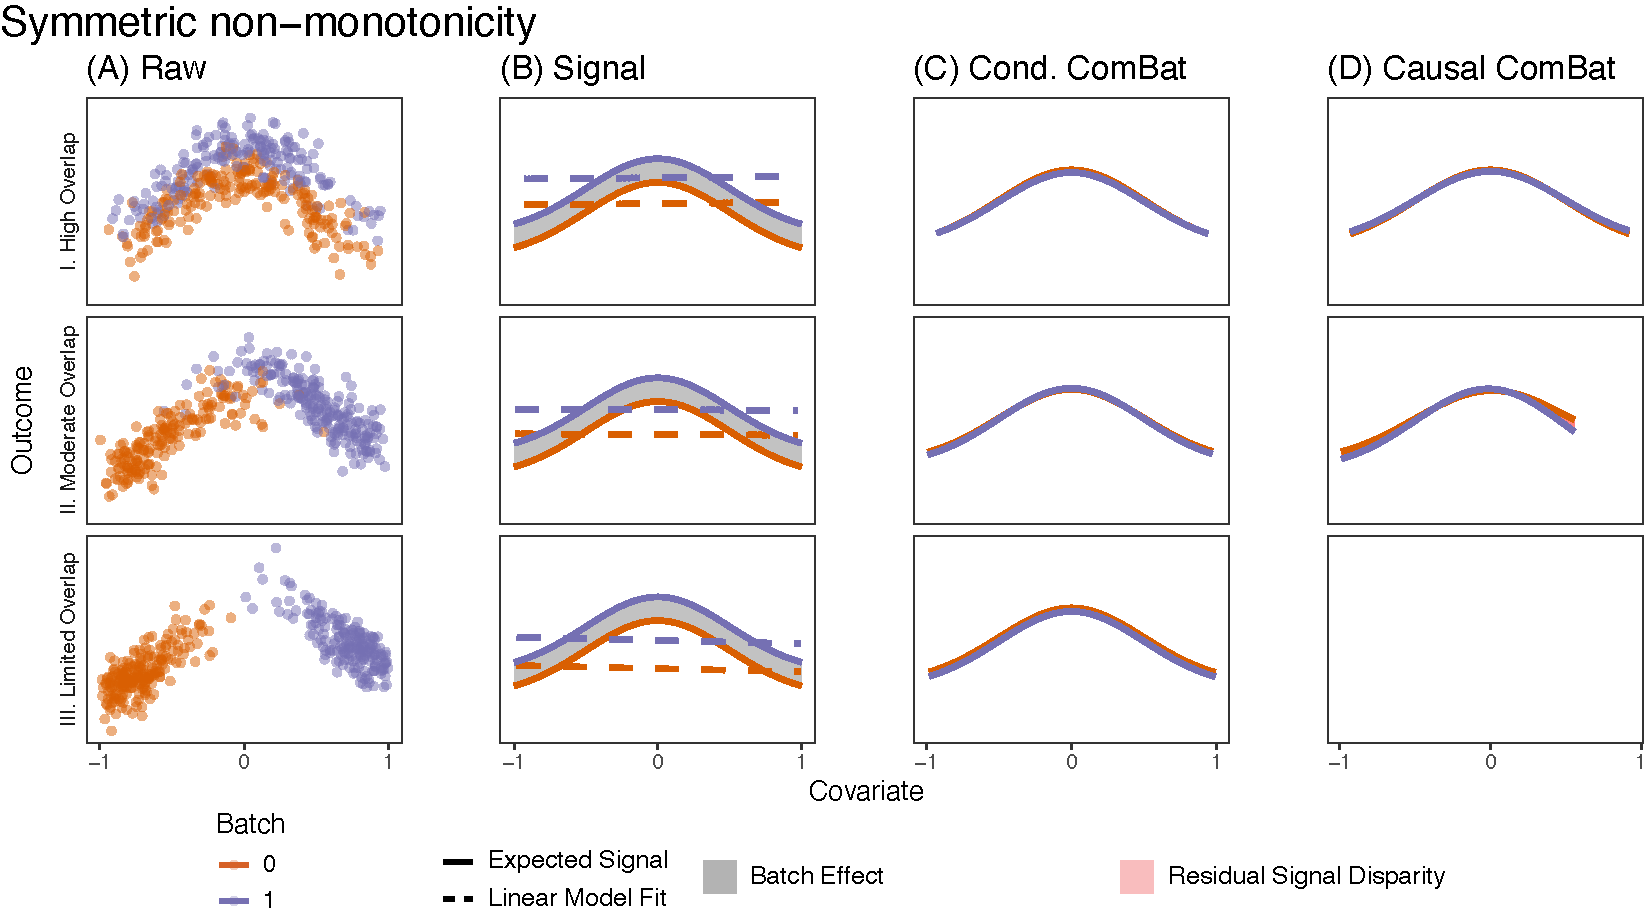
\includegraphics[width=\linewidth]{Figures/Supplement/Simulations/sim_nlin_adjust_nm_sym.pdf}
    \caption{A symmetric non-monotonicity about $x=0$. \ccombat~provides reasonable results when the non-monotonicity and the covariate distributions (for each batch) are symmetric about the same value (here, $x=0$). In high balance the MAAD of \ccombat~and \cccombat~are $0.076$ and $0.051$ (\cccombat~better $67.6\%$ of the time), in moderate balance are $0.179$ and $0.173$ (\cccombat~better $50.9\%$ of the time), and in limited overlap are $0.358$ and $0.289$ (\cccombat~better $66.7\%$ of the time) with \cccombat~only executing in $36$ simulations.}
    \label{fig:sim_nlin_adjust_nm_sym}
\end{figure}

\paragraph*{Asymmetric non-monotonicity} A gaussian non-monotonic relationship between the covariate and the outcome. The outcome is:
\begin{align*}
    Y_i = \varphi\parens*{X_i, \mu=-0.5, \sigma=\frac{1}{2}} + T_i + \frac{1}{2}\epsilon_i.
\end{align*}
We call it ``asymmetric'' because $\mu = -0.5$, which leads to the effect not being symmetric about $x = 0$ (whereas the covariates are, by construction, symmetric about $x=0$). The effectiveness of batch effect correction methods for the asymmetric non-monotonicity setting are shown in Figure \ref{fig:sim_nlin_adjust_nm_asy}.

\begin{figure}[h]
    \centering
    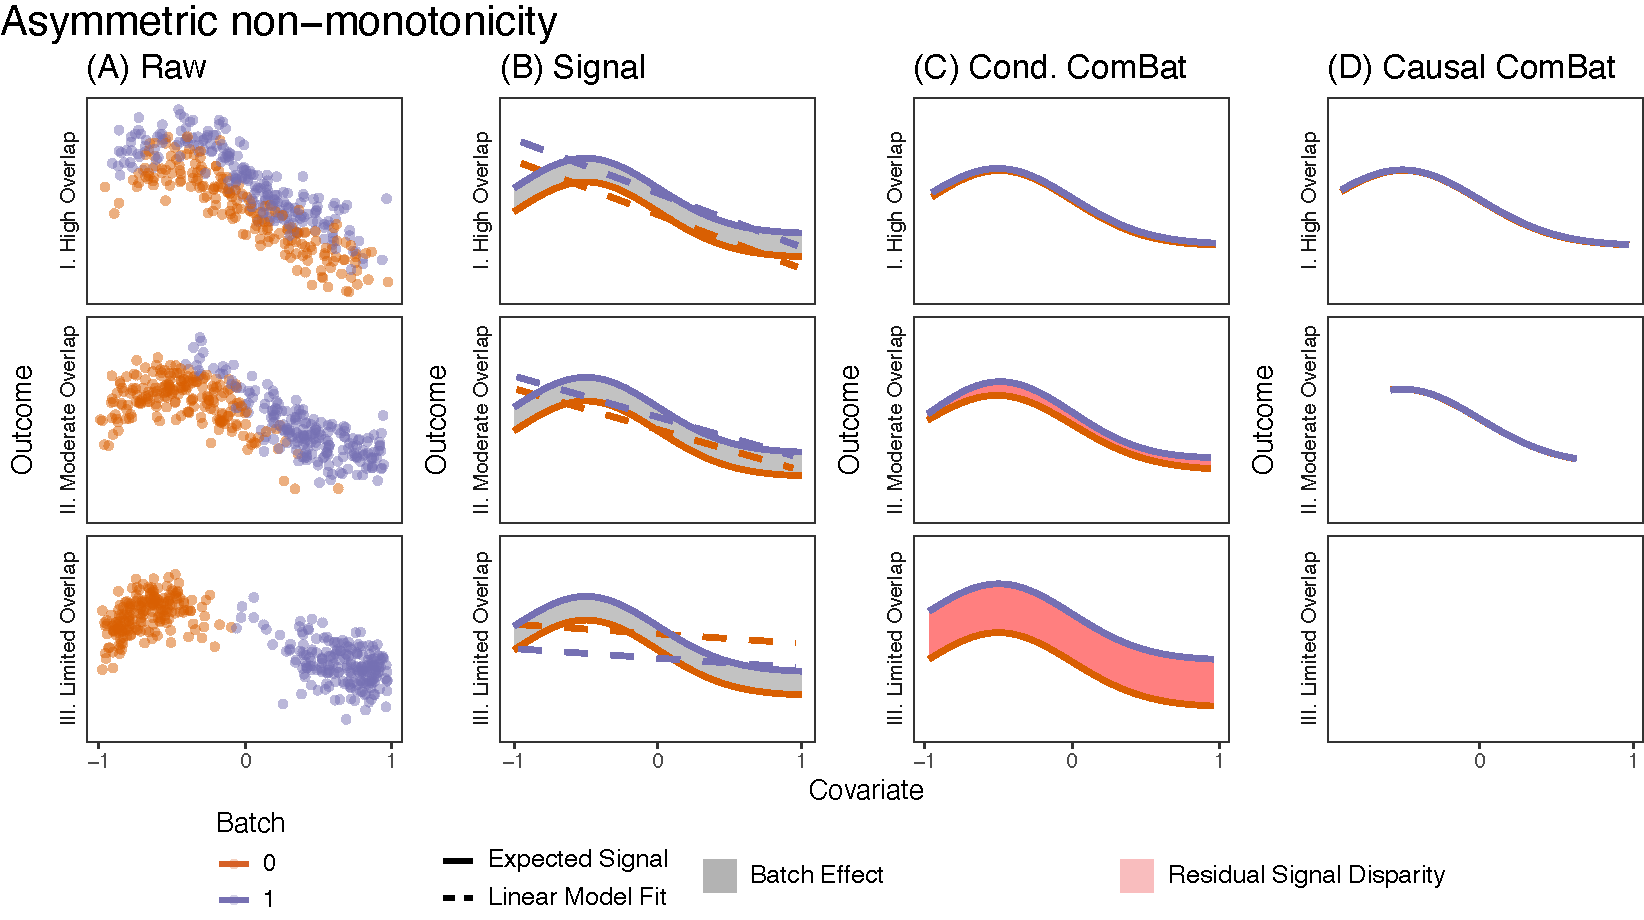
\includegraphics[width=\linewidth]{Figures/Supplement/Simulations/sim_nlin_adjust_nm_asy.pdf}
    \caption{An asymmetric non-monotonicity in which the non-monotonicity is not symmetric about $x=0$, while the covariate distributions (for each batch) are symmetric about $x=0$. \ccombat~ struggles and worsens the batch effect as the covariate balance decreases, while \cccombat~is able to work as long as there are moderate amounts of covariate overlap. In high balance the MAAD of \ccombat~and \cccombat~are $0.0497$ and $0.0421$ (\cccombat~better $59.5\%$ of the time), in moderate balance are $0.074$ and $0.130$ (\cccombat~better $99.7\%$ of the time), and in limited overlap are $2.61$ and $0.407$ (\cccombat~always better) with \cccombat~only executing in $33$ simulations.}
    \label{fig:sim_nlin_adjust_nm_asy}
\end{figure}


\paragraph*{Symmetric non-monotonicity, asymmetric covariates} A gaussian non-monotonic relationship between the covariate and the outcome, and a different covariate distribution from the rest of the simulations. The covariate distribution is:
\begin{align*}
    X_i | T_i = t \distas{d} \begin{cases}
        2\Beta(2, 2) - 1 & t = 0 \\
        2Beta(b, 2) - 1 & t = 1
    \end{cases}
\end{align*}
where $b = 2$, $b=6$, and $b=12$ for the overlap, moderate, and limited conditions, respectively.

The outcome is:
\begin{align*}
    Y_i = \varphi\parens*{X_i, \mu=0, \sigma=\frac{1}{2}} + T_i + \frac{1}{2}\epsilon_i.
\end{align*}
This time, the non-monotonicity is symmetric, but the covariate distributions are increasingly asymmetric. The effectiveness of batch effect correction methods for the asymmetric non-monotonicity setting are shown in Figure \ref{fig:sim_nlin_adjust_nm_sym_asy}.

\begin{figure}[h]
    \centering
    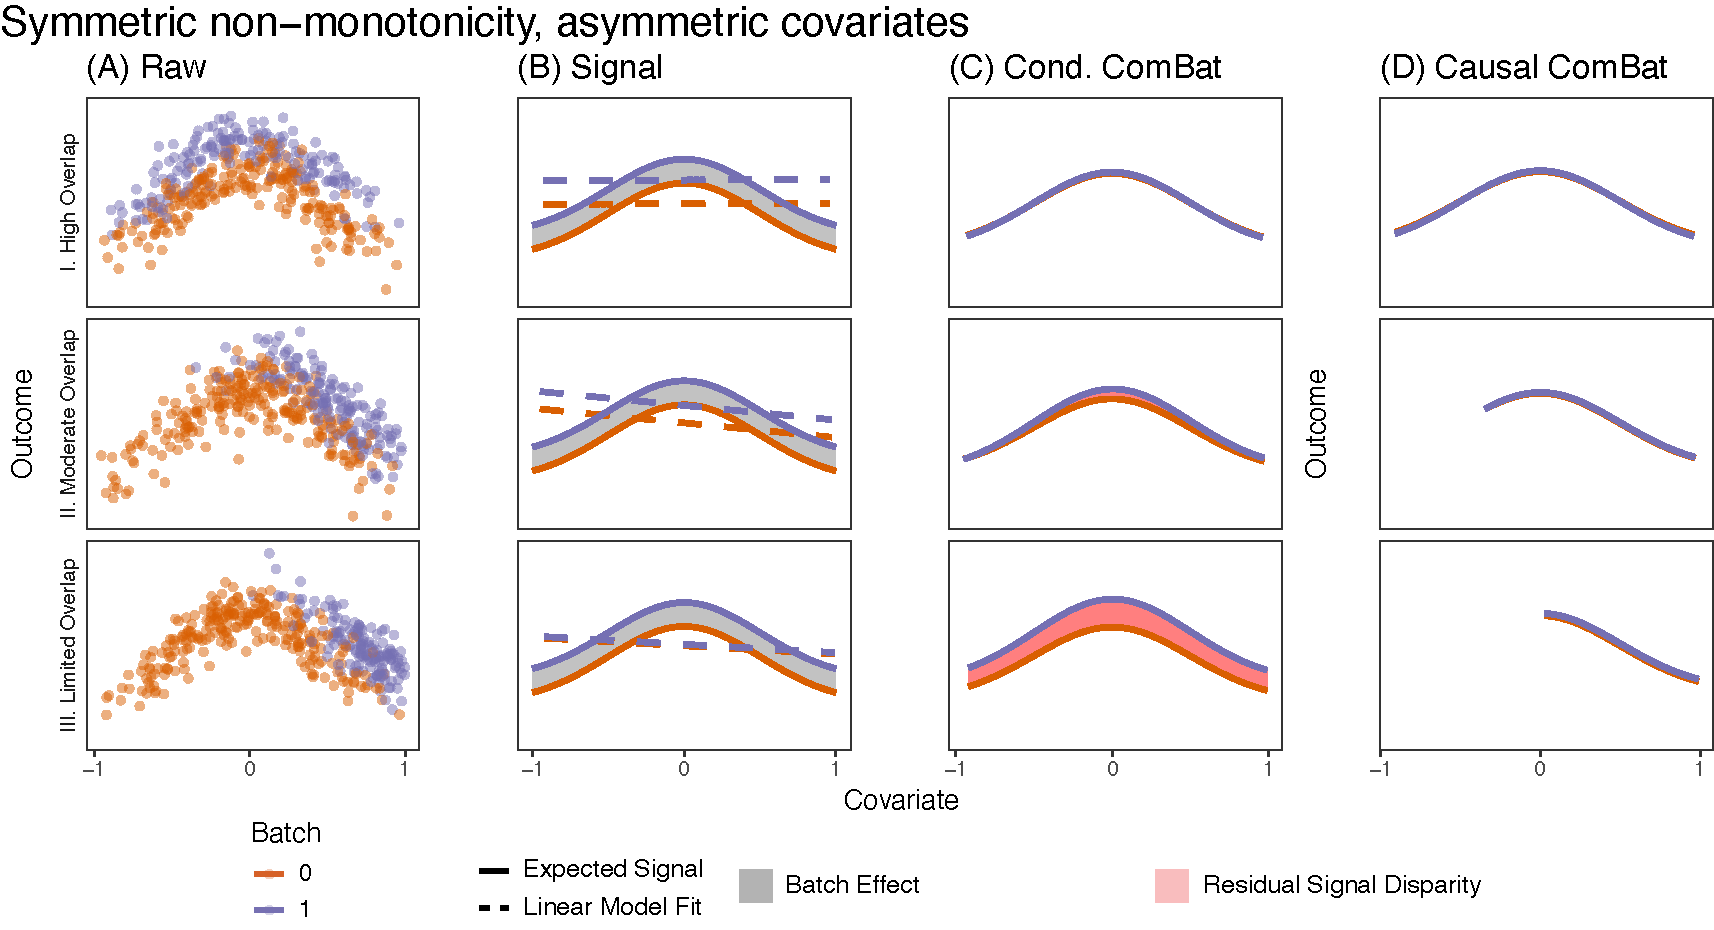
\includegraphics[width=\linewidth]{Figures/Supplement/Simulations/sim_nlin_adjust_nm_sym_asy.pdf}
    \caption{A symmetric non-monotonicity about $x=0$, but the covariate distribution is no longer symmetric about $x=0$. \ccombat~struggles to remove the batch effect and leaves a residual signal disparity, but \cccombat~is able to address the batch effect within a range of covariate overlap. In high balance the MAAD of \ccombat~and \cccombat~are $0.075$ and $0.0506$ (\cccombat~better $65.8\%$ of the time), in moderate balance are $0.181$ and $0.0751$ (\cccombat~better $96.0\%$ of the time), and in limited overlap are $0.84$ and $0.106$ (\cccombat~always better). Due to the fact that the covariate distribution for batches $0$ and $1$ overlap for this simulation, \cccombat~always executes.}
    \label{fig:sim_nlin_adjust_nm_sym_asy}
\end{figure}


\paragraph*{Linear} A linear relationship between the covariate and the outcome. The outcome is:
\begin{align*}
    Y_i = -2\parens*{X_i - 1} + T_i + \frac{1}{2}\epsilon_i.
\end{align*} The effectiveness of batch effect correction methods for the linear setting are shown in Figure \ref{fig:sim_lin_adjust}.

\begin{figure}[h]
    \centering
    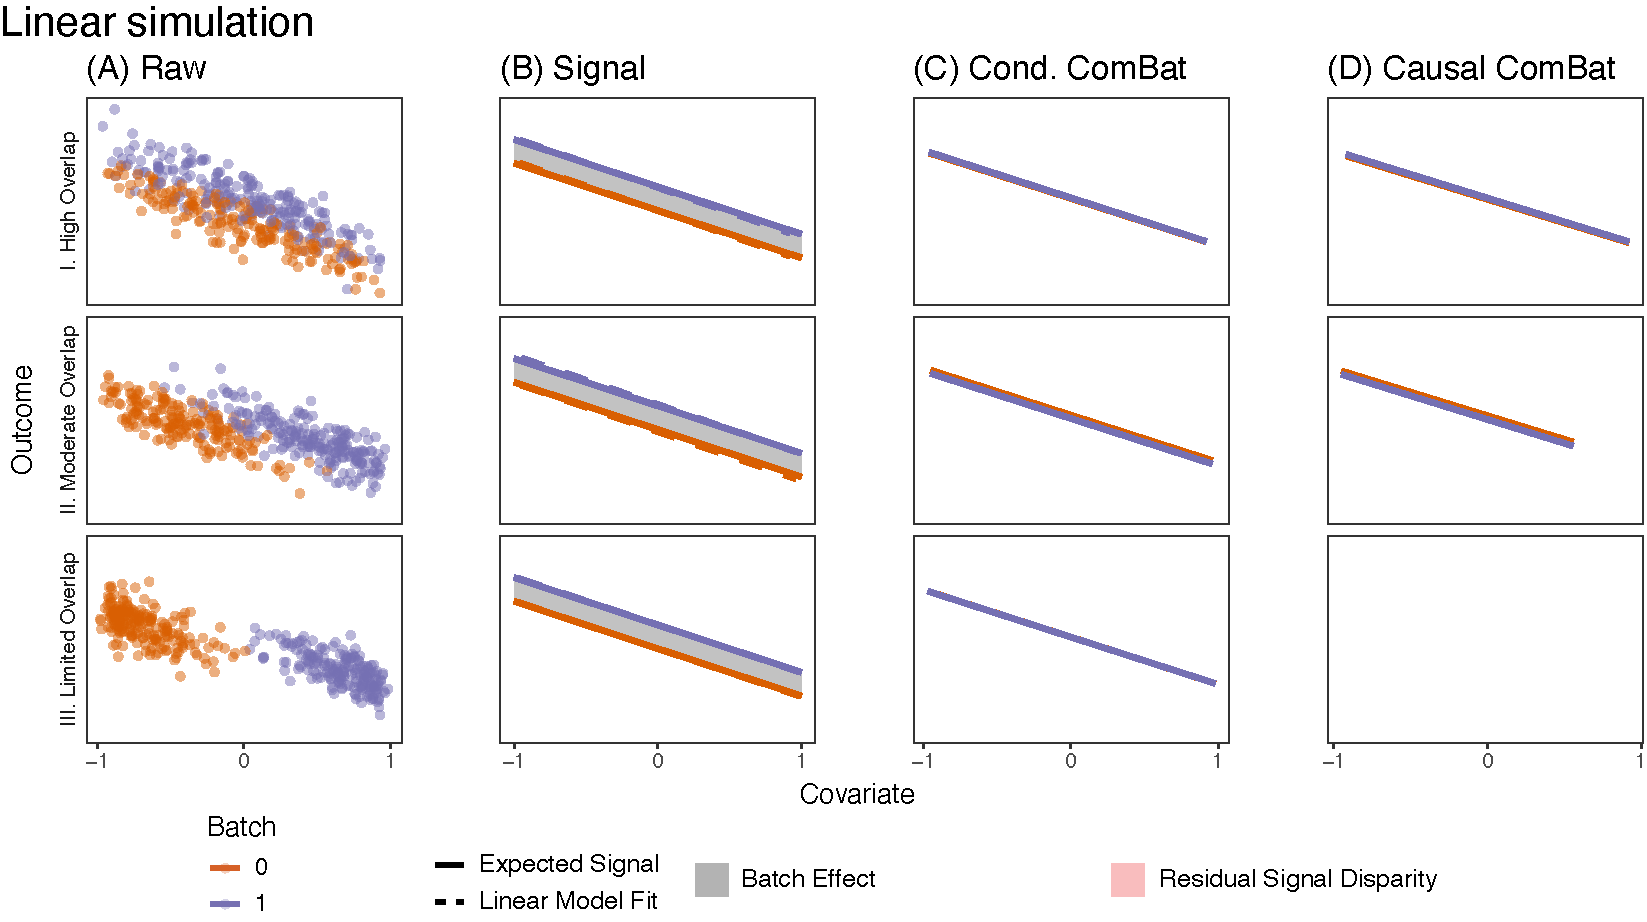
\includegraphics[width=\linewidth]{Figures/Supplement/Simulations/sim_lin_adjust.pdf}
    \caption{A linear simulation in which the assumptions of \ccombat~are perfectly satisfied. In high balance the MAAD of \ccombat~and \cccombat~are $0.035$ and $0.0375$ (\cccombat~better $42.5\%$ of the time), in moderate balance are $0.074$ and $0.113$ (\cccombat~better $33.1\%$ of the time), and in limited overlap are $0.145$ and $0.292$ (\cccombat~better $23.1\%$ of the time) with \cccombat~only executing in $39$ simulations.}
    \label{fig:sim_lin_adjust}
\end{figure}

\subsection{Mean Average Absolute Difference (Mean AAD)}
\label{app:maad}
To evaluate the effectiveness of each batch effect correction technique on simulated data, we compute the true data expected signal for each covariate level; e.g., $\expect{Y_i(t) | x}$ for each batch $t$ and each covariate level $x$. Since $\epsilon_i$ has mean $0$, this would be the quantity:
\begin{align*}
    \expect{Y_i(t) | x} &= f(x) + t,
\end{align*}
where $f$ is the covariate/outcome relationship (possibly incorrectly modeled). Since $x$ is continuous, we compute this value for $x$ across $B=200$ evenly spaced breakpoints for evaluation. Given a set of samples, we train a batch effect correction model, and fit the trained model to the expected signal for each covariate level, leaving us with adjusted expected signal for each batch, which we denote by $V_i(t, x)$. In theory, if the batch effect correction technique removes the batch effect as modeled, $V_i(1, x) \approx V_i(0, x)$ for all $x$. To evaluate each technique, we consider the average absolute difference for each trial $r$ of $1000$ trials:
\begin{align*}
    d_r &= \frac{1}{B} \sum_{x \in \mathcal X}\left|v_i(1, x) - v_i(0, x)\right|,
\end{align*}
and the magnitudes of $d_r$ are annotated in the plots (shaded red boxes) for a single simulation. We compute the mean AAD as:
\begin{align*}
    d &= \frac{1}{r}\sum_{r \in [R]} d_r.
\end{align*}
A value of $0$ corresponds to the batch effect being completely eliminated (the expected signal for each batch after correction is identical), a value of $1$ would equate to the residual disparity between the expected signals being the same as before batch effect correction, and a value $> 1$ corresponds to the residual disparity between the expected signals \textit{exceeding} the original batch effect.

\subsection{Causal \Combat~outperforms Conditional \Combat~on simulated data}

Across all simulations, simulated measurements are collected from an additive gaussian model with either a linear (Figure \ref{fig:sim_lin_adjust}), non-linear (Figure \ref{fig:sim_nlin_adjust}), or non-monotonic (Figure \ref{fig:sim_nlin_adjust_nm_sym}, Figure \ref{fig:sim_nlin_adjust_nm_asy}, and Figure \ref{fig:sim_nlin_adjust_nm_sym_asy}) covariate/outcome relationship, with a batch-specific offset. We performed these simulations for cases where the covariate distributions overlap (row I), moderately overlap (row II), and have limited overlap (row III). When the assumptions between the covariate and the measurements are correct, covariate overlap is irrelevant, as the covariate-specific signal can be extrapolated successfully across the entire range of the covariate. When the assumptions between the covariate and the measurements are incorrect, the batch effect can still be removed, as shown in column (D), when further conditions are satisfied, such as:
\begin{enumerate}[leftmargin=*]
    \item covariate distributions are matched: can be conceptualized as the inaccurate assumptions of the model, in effect, being uniformly \textit{misrepresented} by the model in each of the two batches, which \textit{still} enables a consistent estimate of the batch effect to be estimated and removed. \cccombat~attempts to enforce this approach through matching. We explored the implications of this in Figure \ref{fig:sim_nlin_adjust} and Figure \ref{fig:sim_nlin_adjust_nm_asy}.
    \item the covariate distributions (and the covariate/outcome relationship) are symmetric about the same point: again, the idea here is that intuitively, the the inaccurate assumptions of the model must be uniformly misrepresented by the model in the two batches. This is a pre-hoc condition and relates directly to the specific underlying true veridical signal, and is difficult to exploit practically. We explore the implications of this in Figure \ref{fig:sim_nlin_adjust_nm_sym} and Figure \ref{fig:sim_nlin_adjust_nm_sym_asy}.
\end{enumerate}

As shown in the simulations in Figure \ref{fig:sim_nlin_adjust} and Figure \ref{fig:sim_nlin_adjust_nm_asy}, these artifacts can be arbitrarily large depending on the nature of the incorrect assumption. In these examples, the residual signal disparity introduced by \ccombat~in limited overlap cases (row III) dwarfs the magnitude of the original batch effect, and is of similar magnitude with moderate covariate overlap (row II). 

On the other hand, \cccombat~first pre-aligns the covariate distributions, and even with model misspecifications, is able to successfully remove a batch effect for the subset of the covariate space with sufficient covariate overlap. Importantly, causal strategies \textit{explicitly prohibit} learning about data which falls outside of the region of demographic overlap. When overlap conditions are not met for a portion of the sample space, causal strategies do not do anything, as is typically the case for most of the illustrated similations in the ``Limited Overlap'' condition. In this sense, causal techniques are therefore more conservative for batch effect detection and mitigation. We believe this to be favorable for batch effect detection and mitigation as, in practice, it is effectively impossible to tell whether the implicit or explicit assumptions of the model for batch effect correction~are sufficient or not, and almost impossible for our model to account for all ways a batch effect could manifest in high-dimensional data (such as higher order correlations, non-linearities, variance differences) given a finite sample. This presents an enormous point of caution when applying batch effect removal techniques to high-dimensional datasets with confounding, as it is infeasible to explore whether extrapolatory modeling assumptions are within reason on a dimension-by-dimension (or, higher-order) basis.}

}

\paragraph{Addressing the batch effect}
One way to characterize the batch effect in univariate contexts (and within our simulations) would be analogous to the average treatment effect \cite{Rosenbaum1983Apr}; e.g.:
\begin{align*}
    \text{ATE} = \expect{Y(1) - Y(0)}
\end{align*}
For all simulations, by construction the ATE is $1$ and does not depend on the covariates.

By definition, a difference in the expectations implies that $Y(1) \overset{\mathcal D}{\neq} Y(0)$, and a batch effect is present by Definition \ref{def:causal_batch_informal}.

It is well understood in the statistical literature that for models of the form $Y_i = g(X_i) + \beta T_i + Z_i$ where $Z_i \distas{iid} \Norm{\mu, \Sigma}$, that as long as either the strong ignorability condition \cite{Rosenbaum1983Apr} or $f$ is known, the adjustment factor $\hat\beta_1 - \hat \beta_0$ will be a consistent and unbiased estimate of the ATE \cite{Rosenbaum1983Apr, vdv}. For a non-technical explanation in words, we can obtain reasonable estimates of the ATE in one of three ways (and consequently, account for the batch effect):
\begin{enumerate}[leftmargin=*]
    \item Extrapolation: if we know $g(x)$, then we can ``guess'' what $\expect{Y_i(t)|x}$ looks like for values of $x$ that do not exist in our batch, by appropriate estimation of $g$ via the elements of our dataset that we \textit{do} have. In this case, where the model is linear, extrapolation can be performed by linear regression. Once we have identified $g(x)$, we can extrapolate what $g(x)$ looks like for values of $x$ which fall outside the range of our dataset, as in Figure \ref{fig:sim_lin_adjust}; particularly, noting cells (C).II and (C).III.
    \item Use asymptotics: if we do not know $g(x)$ but we can reasonably assume that the strong ignorability condition holds, we can leverage asymptotic statistics to conclude that we can still adequately estimate the CATE. Proofs of this result can be found in \cite{Rosenbaum1983Apr,Rosenbaum1985}. In this particular case, $X_i \indep T_i$, which implies the strong ignorability condition \cite{Rosenbaum1983Apr}. For more trivial reading specific to the case where $X_i \indep T_i$, see \cite{vdv}. This result is exhibited in the simulations for Figure \ref{fig:sim_nlin_adjust} and Appendix Figure \ref{fig:sim_nlin_adjust_nm_asy} looking at column (D) compared to column (C), and noting that causal pre-processing procedures tend to produce a reasonable result (while non-causal conditional procedures with a model misspecification do not).
    \item The covariate distribution is symmetric about the same point that a non-monotonicity is symmetric: in this extremely special case, we have that $f(x | 1) = f(-x | 0)$, and $f(y(0) | x) = f(y(1) | -x)$ for every $x$. This result is exhibited by way of comparison of Figures \ref{fig:sim_nlin_adjust_nm_sym} and Figure \ref{fig:sim_nlin_adjust_nm_asy}, and noting that while Figure \ref{fig:sim_nlin_adjust_nm_sym}(C).III is able to arrive at a reasonable solution, Figure \ref{fig:sim_nlin_adjust_nm_asy}(C).III does not.
\end{enumerate}
By a similar argument, the estimated batch disparity can also be consistently estimated in either of these contexts. In these cases, removal of the estimated offset associated with the particular batch of a measurement is a reasonable approach to removal of the estimated batch effect.

Simulations in which the assumption about $f(x)$ is incorrect and $X_i$ is distributed conditionally on $T_i$ (and consequently, the strong ignorability condition will not hold), will not necessarily yield a reasonable estimate of the ATE.
}

\section{Overlap of Empirical Covariates}
\label{app:overlap}

The empirical overlap of the covariate distributions is difficult to compute in the case of data without making heavy parametric assumptions. For this reason, we turn to the distribution-free overlapping index \cite{Pastore2019}. The distribution free overlapping index, $\hat v_{kl}$, is computed by first approximating the density of the distribution of the measured covariates for each dataset $D$, $X = (A, S, C)$, where $A$ is a random variable whose realizations $a \in \mathcal A$ are ages, $S$ is a random variable whose realizations $s \in \mathcal S$ are sexes (M or F), and $C$ is a random variable whose realizations $c \in \mathcal C$ denote continent, using the base \texttt{R} function \texttt{stats::density}. The random variable $D$ has realizations $d \in \mathcal D$ whose realizations denote dataset. The density $f\parens*{a| S = s, C = c, D = d}$ is the conditional density of age, conditional on the individual's sex being $s$, continent of measurement being $c$, and dataset being $d$. The mass $\prob{S = s | C = c, D = d}$ is the conditional mass of sex, conditional on the individual's continent of measurement being $c$, and dataset being $d$. Finally, the mass $\prob{C = c | D = d}$ represents the conditional mass of an individual's continent of measurement being $c$, conditional on the dataset being $d$ ($0$ or $1$ for all $d$, since all individuals from dataset $d$ are either measured on continent $c$ or not). An estimate of the overlap between the two densities, $\hat v_{kl}$ between datasets $k$ and $l$, is computed using the formula:
\begin{align*}
    \hat v_{kl} &= \sum_{c \in \mathcal C}\min\parens*{\hat {\mathbb P}\parens*{C = c | D = k}, \hat{\mathbb P}\parens*{C = c | D = l}}\sum_{s \in \set*{\text M, \text F}}\min\parens*{\hat{\mathbb P}\parens*{S = s | C = c, D = k},\hat {\mathbb P}\parens*{S = s | C = c, D = l}}\bigg[ \\
    &\undereq\integral{\mathcal A}{}{\min\parens*{\hat f\parens*{a | S = s, C = c, D = k}, \hat f\parens*{a | S = s, C = c, D = l}}}{a}\bigg]
\end{align*}
which is obtained via numerical quadrature.

Intuitively, this can be conceptualized as representing the mass of the "area under the curve" which is shared by the two densities for datasets $k$ and $l$.

\begin{figure}[h!]
    \centering
    \includegraphics[width=\linewidth]{Figures/Supplement/ov_app.pdf}
    \caption{\textbf{The overlap of the empirical covariate distributions for the American Clique, before and after adjustment}. \textbf{(A)} The empirical distributions of the covariates before adjustment. \textbf{(B)} The empirical overlap of the covariate distributions after the adjustment procedure is applied, as discussed in Appendix \ref{app:cross_effect}.}
    \label{fig:overlap}
\end{figure}

\begin{figure}[h!]
    \centering
    \includegraphics[width=\linewidth]{Figures/Supplement/mega_overlap.pdf}
    \caption{\textcolor{black}{\textbf{The overlap of the empirical covariate distributions for two mega-studies.} \textbf{(A)} The empirical distribution of covariates. \textbf{(B)} The overlap of covariate distributions given by the distribution-free overlapping index for ABIDE mega-study \cite{di2014autism, di2017enhancing}. \textbf{(C)} The overlap of covariate distributions given by the distribution-free overlapping index for the SRPBS mega-study. \cite{Yamashita2019Apr}. Like for the CoRR mega-study, while several pairs of sites have overlapping demographic distributions, many of the sites have extremely poor overlap in both mega-studies. In these cases, attempts to normalize for batch effects using model-based approaches like Conditional \Combat~would be subject to the pitfalls of Figure \ref{fig:sim_nlin_adjust}, Appendix \ref{fig:sim_nlin_adjust_nm_asy}, or Appendix Figure \ref{fig:sim_nlin_adjust_nm_sym_asy} if modeling assumptions are not reasonable.}}
    \label{fig:overlap2}
\end{figure}

\subsubsection{Batch Effects are reduced with Causal \Combat}

Here we investigate batch effects before and after correction. Figure  \ref{fig:site_hists} shows average connectomes from the MRN1 and IBATRT studies. With no correction, while the average connectomes appear similar between the two studies, a difference between the average connectomes is present (bottom row). Three different batch effect mitigation strategies ($Z$-scoring across features within a single batch, \Combat, and Causal \Combat) all appear to eliminate the differences between the average connectomes. $Z$-scoring has disrupted fundamental topological properties of the human connectome, as explored in detail in Appendix \ref{app:topological}. For this reason, we do not consider $Z$-scoring going forward, and focus instead on variations of the \Combat~procedure.

\begin{figure}[h!]
    \centering
    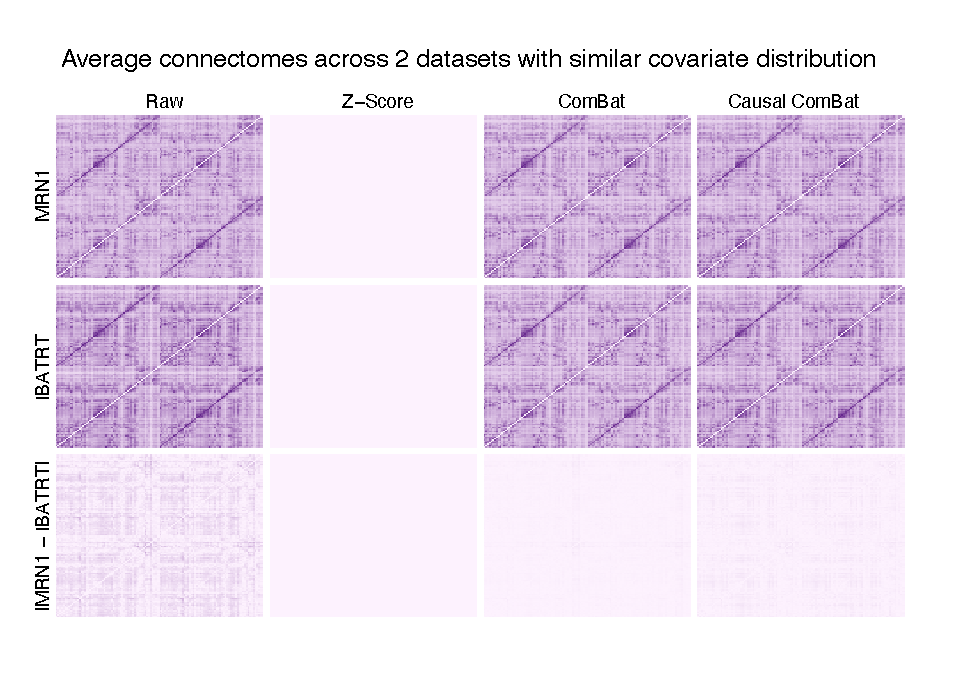
\includegraphics[width=.9\linewidth]{Figures/Content/site_effect_jk_2b.pdf}
    \caption{\textbf{Distribution of Detected Effects Before and After Correction}. A comparison of the average connectomes from two studies from the same continent, with similar sex and age distributions conditional on sex. While the \textit{Raw} average connectomes appear similar, the absolute difference between the two is appreciable. All of the three adjustment strategies reduce the absolute difference between the average connectomes for the two batches.}
    %\textbf{(B)} The difference between the average male and female connectome in the NYU2 study, compared to the difference between the average male connectome from the NYU2 study and the Utah1 study (all female). \Combat~has eliminated the sex disparity in favor of making average connectomes similar across studies.  \textbf{(C)} The difference between the average connectomes in the NYU2 study and the IBATRT study, across the raw, \Combat, and Causal \Combat~connectomes. Causal \Combat~has increased the disparity between the NYU2 study and the IBATRT study.}
    \label{fig:site_hists}
\end{figure}

\section{\Combat\ Preserves Topological Properties of fMRI Connectomes}
\label{app:topological}
% say Z-Score stuff first
The presence of two prominent topological \textit{signal effects} in human connectomes, homophily  and homotopy, are investigated in Figure \ref{fig:site_individual}. 
% avoid stuff like this
The left column of Figure \ref{fig:site_individual}A looks at the edges comprising these two disparate community structures. When edges are sorted by hemisphere, the homophilic effect is characterized by a modular two-block structure, with higher connectivity in the lower left and upper right blocks (dark red) than in the two off-diagonal blocks (pink). The homotopic effect is characterized by edges in the off-diagonal band (dark blue) showing higher connectivity than other edges within the connectome (light blue). The right column of Figure \ref{fig:site_individual}A looks at a single individual's connectome from the NYU2 study before and after correction. The homotopic property appears to be  preserved in only the \Combat\ connectomes, whereas $Z$-scored connectomes do not appear to preserve this property. In Figure \ref{fig:site_individual}B, these two properties are examined statistically for the individuals from the American Clique (Mann-Whitney $U$ Statistic, see Methods \ref{app:control} for details). Points falling along the diagonal line $y=x$ tend to have a similar signal effect before and after batch correction. Whereas \Combat~ strategies tend to preserve the homophilic and homotopic effects, $Z$-scoring tends to decrease these two topological properties of functional connectomes. This is noted by the fact that the majority of the points for $Z$-scoring across both effects tend to fall below the $y=x$ line, indicating that the effect size after $Z$-scoring is lower than the effect size in the raw connectomes.


\begin{figure}[h!]
    \centering
    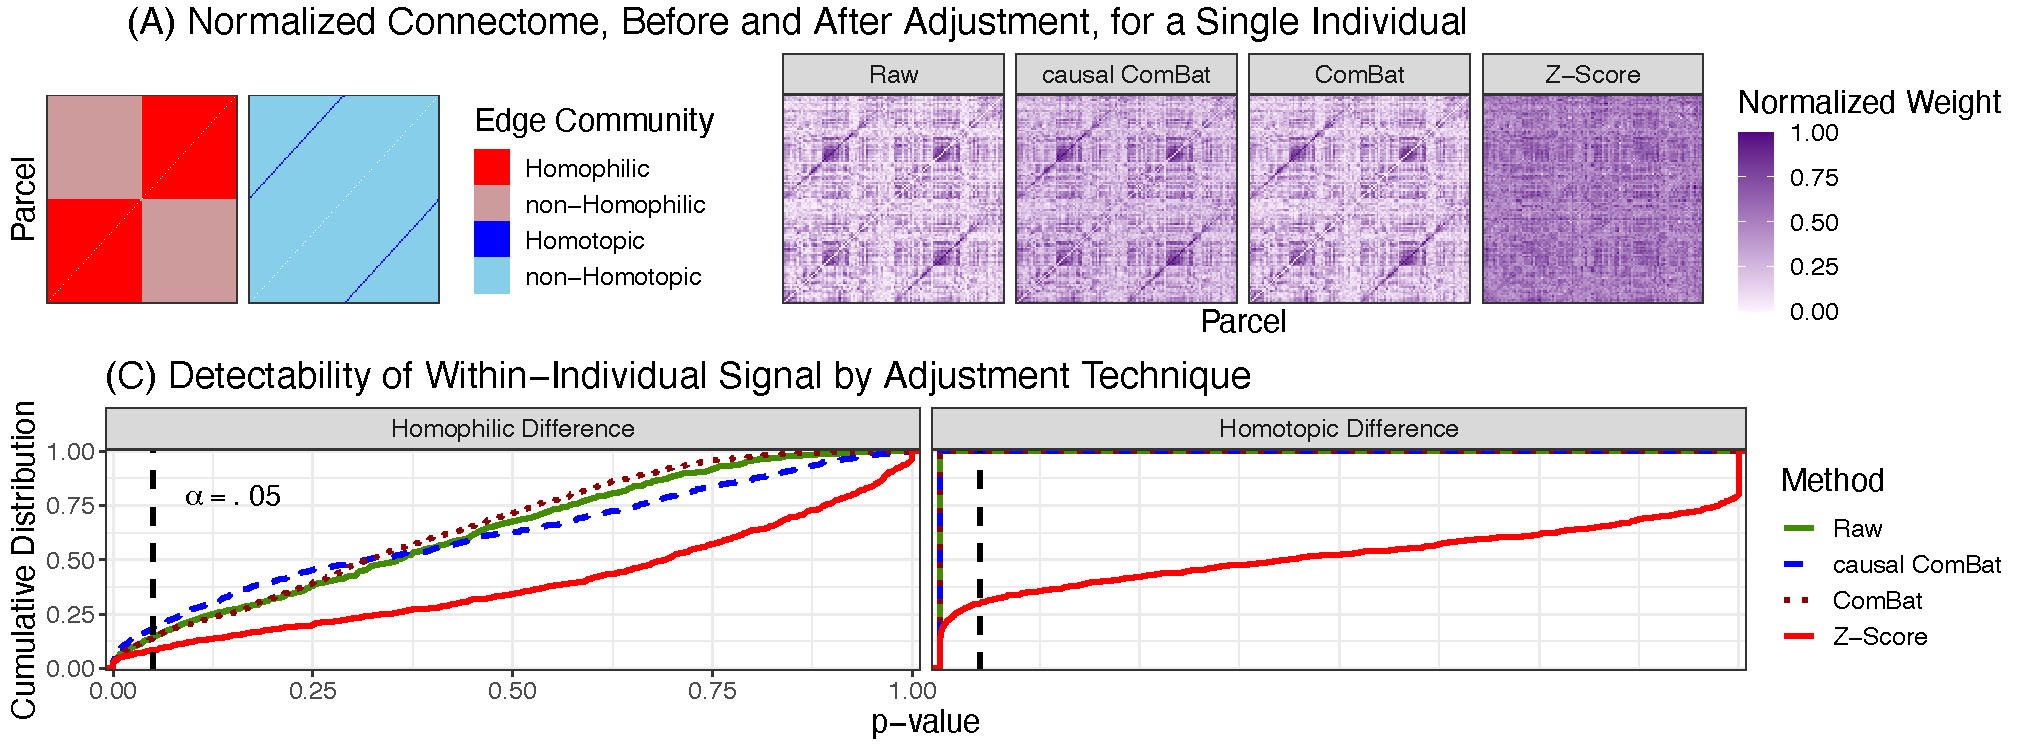
\includegraphics[width=\linewidth]{Figures/Supplement/Signal.png}
    \caption{\textbf{Preservation of Topological Properties of Connectomes after Batch Correction}. The presence of topological effects is explored in the context of the homophilic and homotopic differences in connectivity in the American Clique. \textbf{(A)} (\textit{Left}) A map indicating which edges are associated with homophilic/non-homophilic or homotopic/non-homotopic edge communities. %We look at connectomes only from those in which an adjusted site effect could be removed, from the American Clique \ref{sec:corr_descr}. 
    (\textit{Right}) The edge-weight normalized connectome associated with a single individual from the NYU2 study using each removal strategy. % The adjusted \texttt{ComBat} connectome appears to capture the qualitative properties of the raw connectome. 
    \textbf{(B)} A scatter plot, showing the effect size (Mann-Whitney $U$ Statistic) before (x axis) and after (y axis) the indicated Batch Effect Correction Method.
    % The Wilcoxon Rank-Sum Test is used to test whether the edge weights within the Homophilic/Homotopic edge community exceed those of the non-Homophilic/non-Homotopic community. \texttt{ComBat} tends to preserve the detectability of within-individual signal, whereas \textit{Ranking} and \textit{Z-Scoring} do not. 
    }
    \label{fig:site_individual}
\end{figure}

\begin{figure}[h!]
    \centering
    \includegraphics[width=\linewidth]{Figures/Supplement/top_hist.pdf}
    \caption{Histogram and rug plot indicating the empirical distribution of the normalized edge weights associated with each of the four edge communities for a single individual's connectome.}
    \label{fig:top_hist}
\end{figure}

Figure \ref{fig:top_hist} explores the distribution of edge weights within these two community structures before and after correction. The conclusions are similar in that Causal \Combat\ and \Combat\ preserve the property that the homotopic edges have far higher connectivity than non-homotopic edges. 

\end{document}



